\chapter{ಕೆಲವು ವಿಶೇಷ ಮಾಯಾಚೌಕಗಳು}

\section*{VIII. 1. $8 \times 8$ ಮನೆಗಳ ಒಂದು ವಿಶಿಷ್ಟ ಮಾಯಾಚೌಕ :}

\section*{VIII. $8 \times 8$ ಮನೆಗಳ ಒಂದು ವಿಶಿಷ್ಟ ಮಾಯಾಚೌಕ :}
\begin{figure}[H]
<<<<<<< HEAD
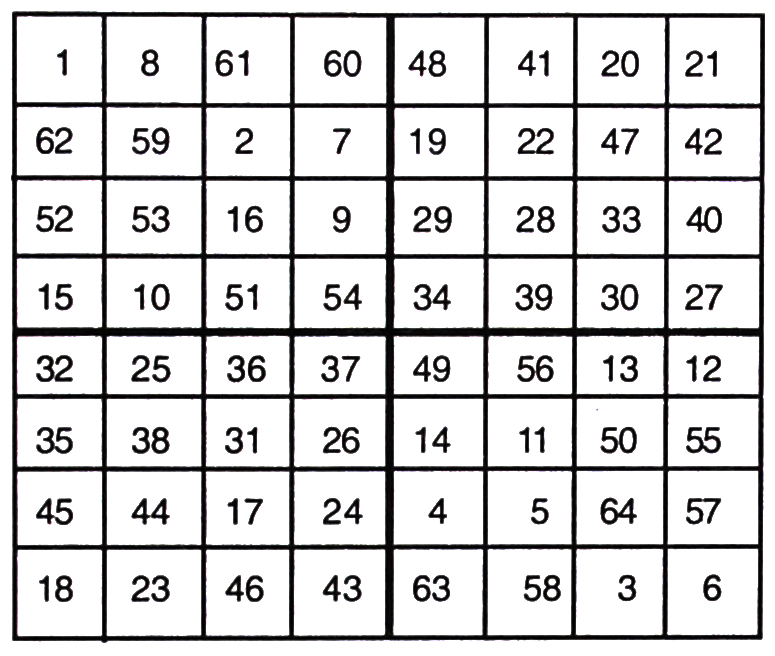
\includegraphics{src/figures/chap7/fig7-1.jpg}
=======
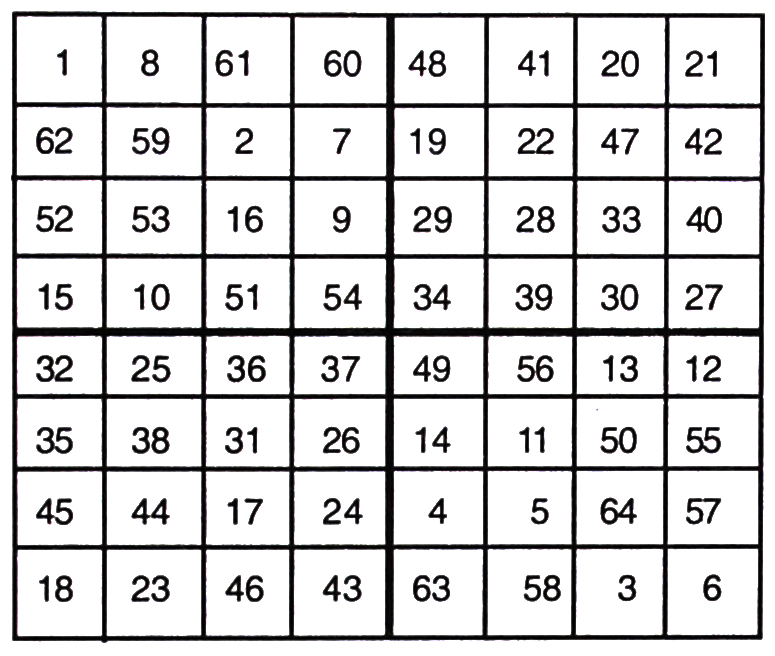
\includegraphics[scale=0.8]{src/figures/chap7/fig7.1.jpg}
>>>>>>> 6489d29d7c8981e9d16559f9e9427e431d3af0bd
\end{figure}

\begin{itemize}
	\item 1ರಿಂದ 64 ಕ್ರಮಾಗತ ಸಂಖ್ಯೆಗಳನ್ನು ಬಳಸಿದೆ.
	\item ಅಡ್ಡಸಾಲು, ಕಂಭಸಾಲು ಕರ್ಣಗಳ ಮನೆಗಳಲ್ಲಿರುವ ಸಂಖ್ಯೆಗಳ ಮೊತ್ತ 260
	\item ಚೌಕವನ್ನು 4 ಸಮಭಾಗಗಳಾಗಿ ವಿಭಾಗಿಸಿದಾಗ ಲಭಿಸುವ ನಾಲ್ಕು $4 \times 4$ ಚೌಕಗಳೂ ಮಾಯಾಚೌಕಗಳೇ.
	\item ಅಡ್ಡಸಾಲು, ಕಂಭಸಾಲು, ಕರ್ಣಗಳ ಸಂಖ್ಯೆಗಳನ್ನು ಪರ್ಯಾಯ (ಒಂದು\break ಬಿಟ್ಟು ಒಂದು)ವಾಗಿ ತೆಗೆದುಕೊಂಡು ಕೂಡಿಸಿದರೆ ಮೊತ್ತ 130. (ಉದಾ: 1+16+49+64=130, 8+53+25+44=130)
	\item ಚೌಕವನ್ನು $2 \times 2$ ಮನೆಗಳ 16 ಸಮಭಾಗಗಳನ್ನಾಗಿ ಮಾಡಿದರೆ, ಪ್ರತಿ $2 \times 2$ ಚೌಕದ ಸಂಖ್ಯೆಗಳ ಮೊತ್ತ 130.

	ಉದಾ : 1+8+62+59, 17+24+46+43, 33+40+30+27 ಇತ್ಯಾದಿ
	\item ಇದು ಒಂದು ಮಾಯಾಘನವೂ ಆಗಿದೆ. (ಪುಟ 104-105 ನೋಡಿ) ಎಡ\break ಮೇಲ್ಭಾಗದ $4 \times 4$ರ ಚೌಕದಿಂದ ಪ್ರಾರಂಭಿಸಿ, ಪ್ರದಕ್ಷಿಣವಾಗಿ ಚೌಕಗಳನ್ನು ಆಯ್ದು, ಒಂದರ ಕೆಳಗೆ ಒಂದು ಬರುವಂತೆ ಜೋಡಿಸಿದರೆ $4 \times 4 \times 4$ ಮಾಯಾ ಘನ\break ದೊರಕುತ್ತದೆ. ಎಲ್ಲ ಪಾರ್ಶ್ವಗಳ ಅಡ್ಡಸಾಲು, ಕಂಭಸಾಲು, ಕರ್ಣಗಳ ಸಂಖ್ಯೆಗಳ\break ಮೊತ್ತ 130.
\end{itemize}

\smallskip

\textbf{VIII. 2.} ಮಾಯಾಚೌಕಗಳ ಲೋಕದಲ್ಲಿ ಅಮೆರಿಕದ ಬೆಂಜಮಿನ್ ಫ್ರಾಂಕ್ಲಿನ್ನದು ಬಹಳ ಪ್ರಸಿದ್ಧ ಹೆಸರು. ತನ್ನ ಕಾಲದಲ್ಲಿ (1706-1790) ಅಧ್ಯಕ್ಷ ಜಾರ್ಜ್ ವಾಷಿಂಗ್ಟನ್ರನ್ನು\break ಬಿಟ್ಟರೆ ಅಮೇರಿಕಾದ ಅತಿ ಪ್ರಖ್ಯಾತ ವ್ಯಕ್ತಿಯಾಗಿದ್ದವನು. ಆತನದು ಬಹುಮುಖ ಪ್ರತಿಭೆ,\break ವಿಜ್ಞಾನಿ, ಸಂಶೋಧಕ, ಮುತ್ಸದ್ಧಿ, ಮುದ್ರಕ, ದಾರ್ಶನಿಕ, ಸಂಗೀತಗಾರ ಮತ್ತು ಅರ್ಥ\-ಶಾಸ್ತ್ರಜ್ಞನಾಗಿದ್ದವ. ಮಾಯಾಚೌಕ ಅವನ ಹವ್ಯಾಸ. ಅವನು ರಚಿಸಿದ ಅನೇಕ ಮಾಯಾಚೌಕಗಳಲ್ಲಿ ಈ ಕೆಳಗಿನದು ಒಂದು.
\begin{figure}[H]
<<<<<<< HEAD
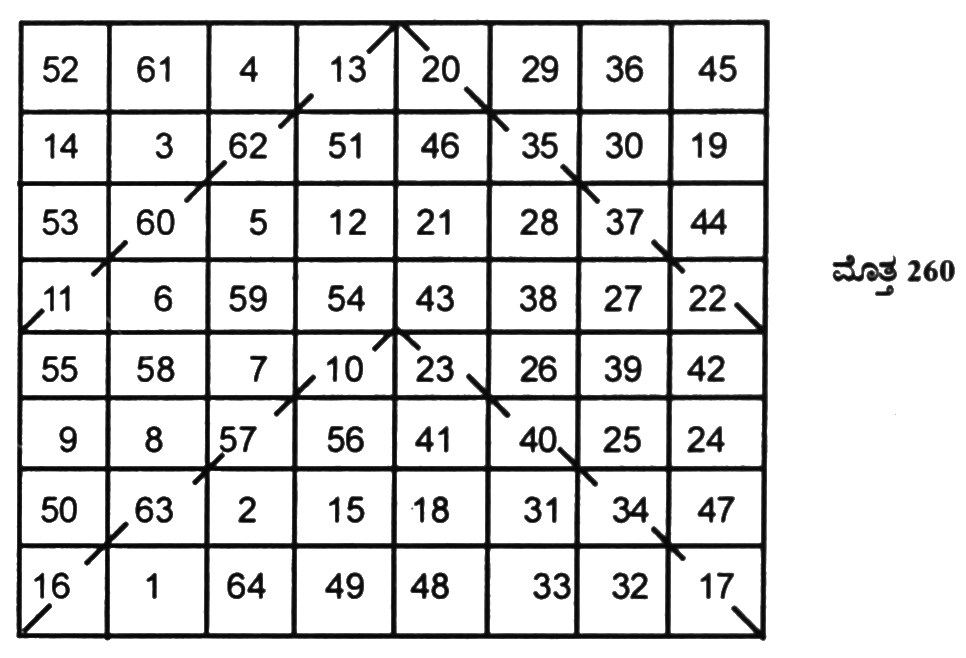
\includegraphics{src/figures/chap7/fig7-2.jpg}
=======
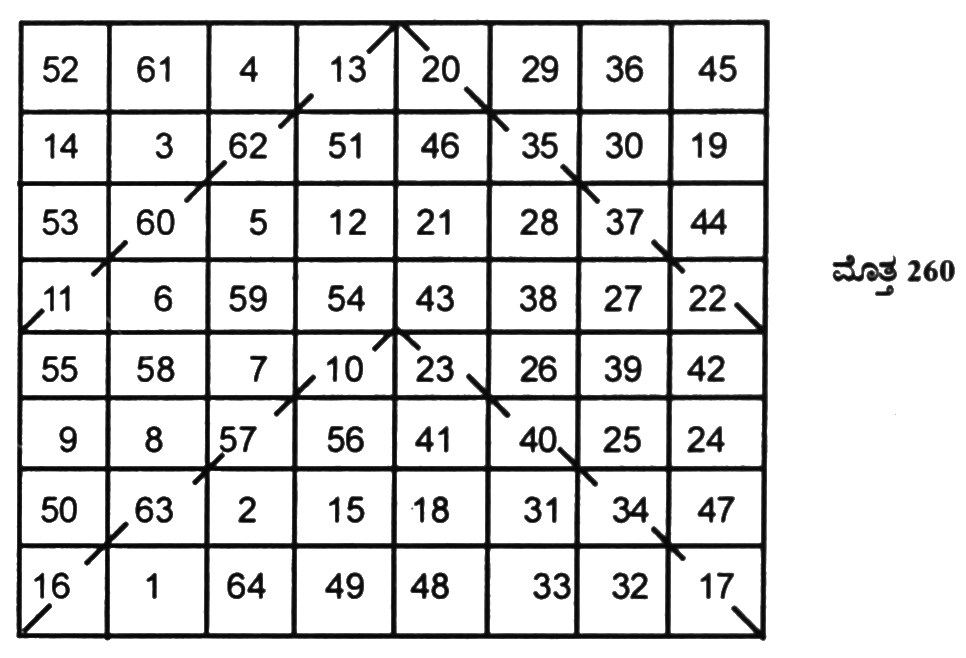
\includegraphics[scale=0.8]{src/figures/chap7/fig7.2.jpg}
>>>>>>> 6489d29d7c8981e9d16559f9e9427e431d3af0bd
\end{figure}

\begin{itemize}
	\item ಅಡ್ಡಸಾಲು, ಕಂಭಸಾಲುಗಳ ಸಂಖ್ಯೆಗಳ ಮೊತ್ತ 260. ಕರ್ಣಗಳದ್ದು ಬೇರೆ.
	\item ನಾಲ್ಕು ಸಮಭಾಗ ಮಾಡಿದರೆ ಆ ನಾಲ್ಕೂ ಮಾಯಾಚೌಕಗಳೇ. (ಕರ್ಣ ಹೊರತು\-ಪಡಿಸಿ)
	\item ಯಾವುದೇ $2 \times 2$ ಚೌಕದ ಸಂಖ್ಯೆಗಳ ಮೊತ್ತ 130
	\item ಯಾವ ಪಕ್ಕದಿಂದಲಾದರೂ ಓರೆಯಾಗಿ 4ಮನೆ ಹೋಗಿ, 4 ಮನೆಗಳನ್ನು ಓರೆ\-ಯಾಗಿ ಇಳಿದರೆ, ಆ ಮನೆಗಳ ಸಂಖ್ಯೆಗಳ ಮೊತ್ತ 260. ಚಿತ್ರದಲ್ಲಿ ಚಿಕ್ಕಗೀಟು ಹಾಕಿರುವ ಮನೆಗಳನ್ನು ಗಮನಿಸಿ.
	\item ಕೇಂದ್ರ ಬಿಂದುವಿನಿಂದ ಸಮಾನ ದೂರದಲ್ಲಿರುವ ಯಾವುದೇ ನಾಲ್ಕು ಸಂಖ್ಯೆಗಳ ಮೊತ್ತ 130. ಉದಾ: 5+28+40+57=130; 3+30+34+63=130; 52+45+17+16=130; 54+43+23+10=130; 1+61+36+32=130 ಇತ್ಯಾದಿ
	\item ಸಂಖ್ಯೆಗಳನ್ನು ಸಮಮಿತಿ (Symmetry)ಯಲ್ಲಿ ತೆಗೆದುಕೊಂಡಾಗ, ಅಂತಹ 8\break ಸಂಖ್ಯೆಗಳ ಮೊತ್ತ 260.
\end{itemize}
ಈ ಕೆಳಗೆ ಕೆಲವು ಮನೆಗಳನ್ನು ಮಸುಕು ಮಾಡಿದೆ. ಆ ಮನೆಗಳಿಗೆ ಅನುರೂಪ ಮನೆಗಳಲ್ಲಿನ ಸಂಖ್ಯೆಗಳ ಮೊತ್ತ 260.
\begin{figure}[H]
<<<<<<< HEAD
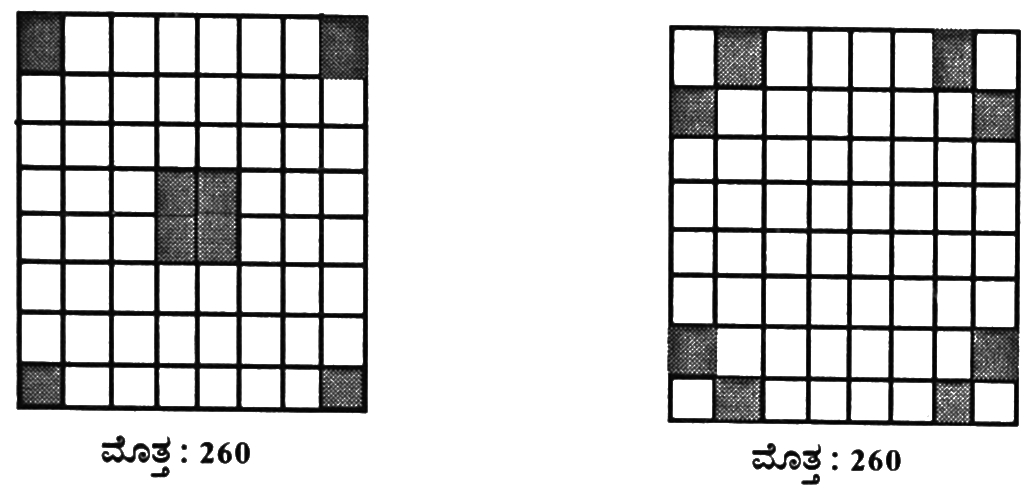
\includegraphics{src/figures/chap7/fig7-3.jpg}
\end{figure}
\begin{figure}[H]
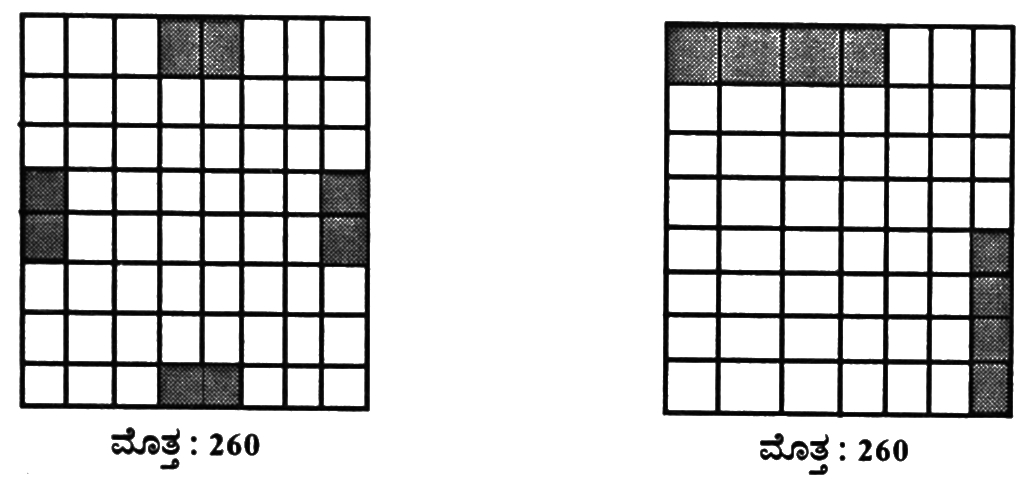
\includegraphics{src/figures/chap7/fig7-4.jpg}
\end{figure}
\begin{figure}[H]
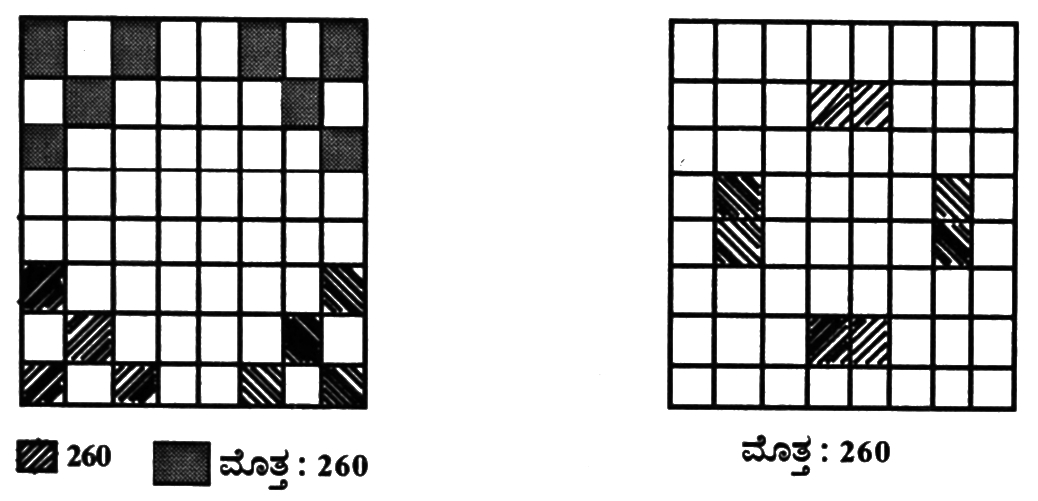
\includegraphics{src/figures/chap7/fig7-5.jpg}
\end{figure}
\begin{figure}[H]
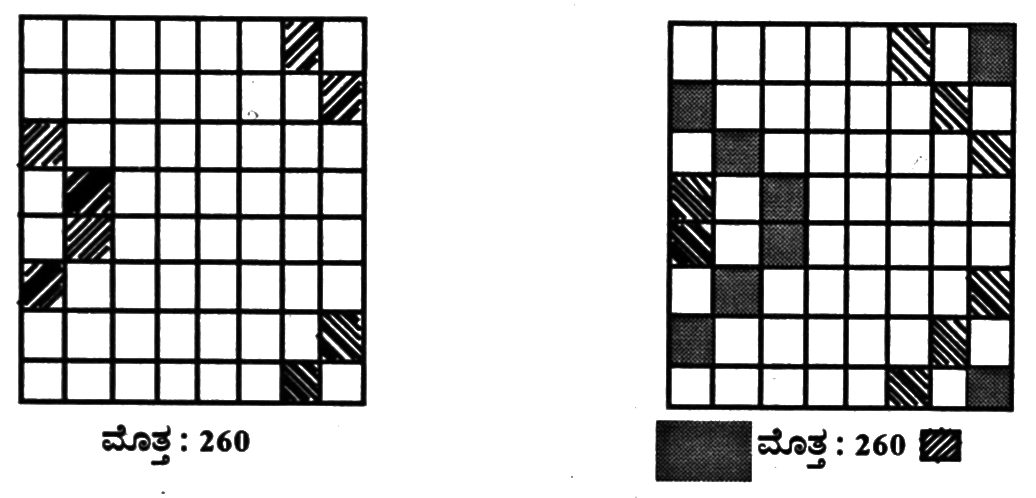
\includegraphics{src/figures/chap7/fig7-6.jpg}
=======
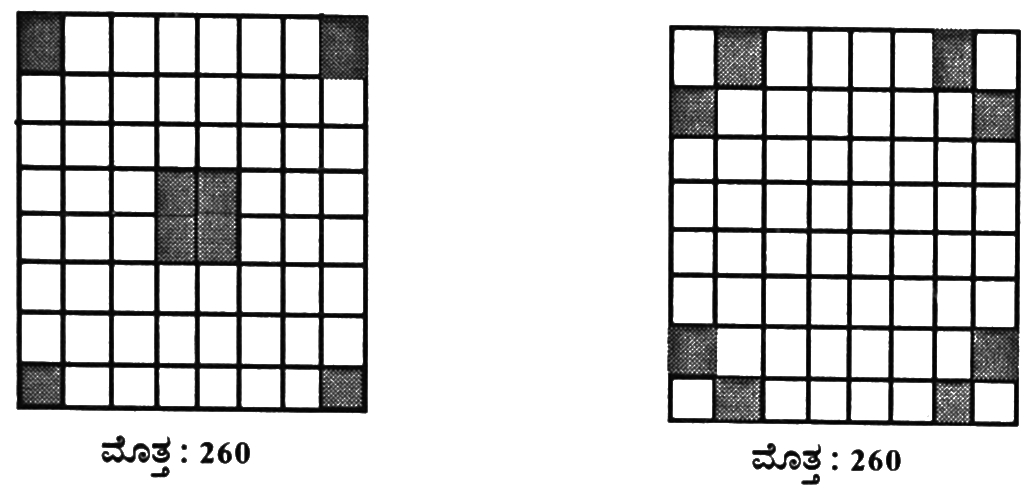
\includegraphics[scale=0.85]{src/figures/chap7/fig7.3.jpg}\\
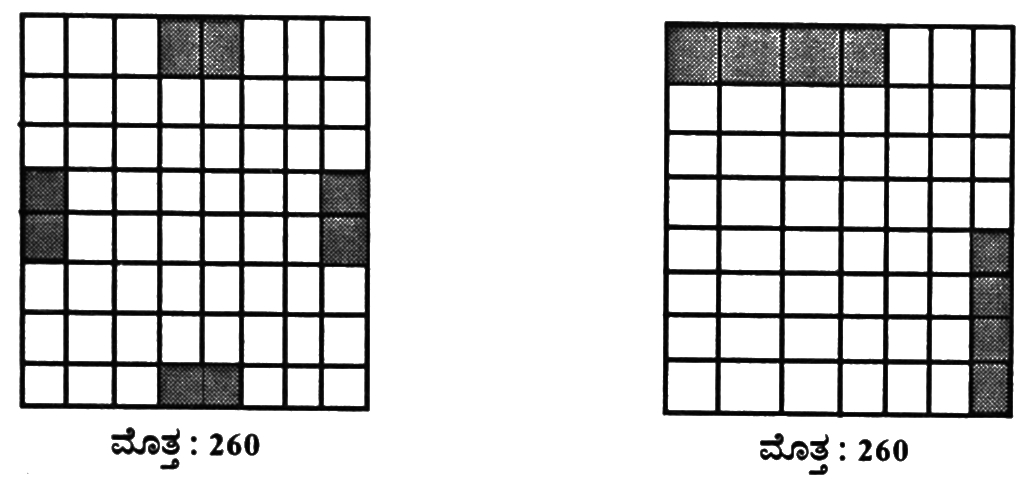
\includegraphics[scale=0.85]{src/figures/chap7/fig7.4.jpg}\\
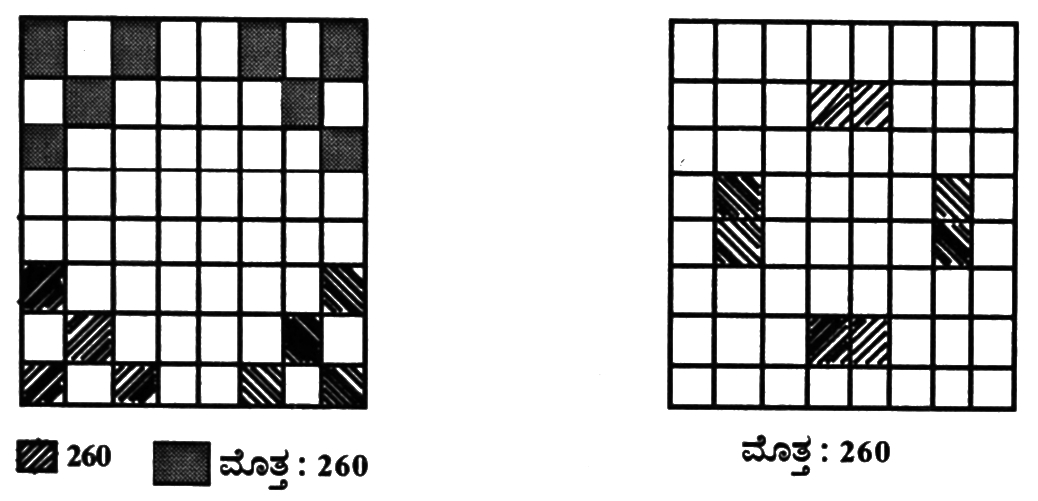
\includegraphics[scale=0.85]{src/figures/chap7/fig7.5.jpg}\\
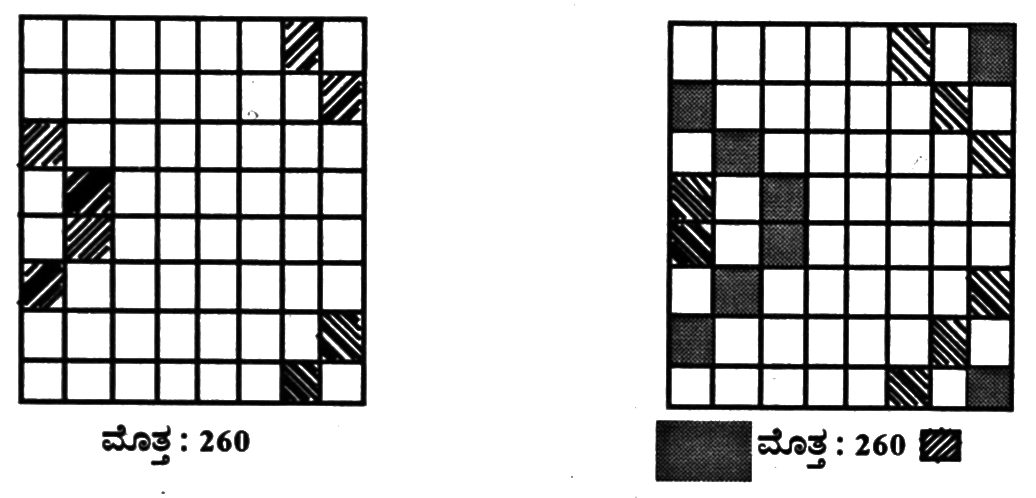
\includegraphics[scale=0.85]{src/figures/chap7/fig7.6.jpg}
>>>>>>> 6489d29d7c8981e9d16559f9e9427e431d3af0bd
\end{figure}

\textbf{VIII. 3.} ಈ $16 \times 16$ ಮಾಯಾಚೌಕವು ಮಾಯಾಚೌಕಗಳಲ್ಲೇ ಅತಿ ವಿಶಿಷ್ಟ ಎಂಬ ಹೆಸರು ಪಡೆದಿದೆ. ಇದನ್ನು ರಚಿಸಿದವರು ಅಮೆರಿಕೆಯ ಬೆಂಜಮಿನ್ ಫ್ರಾಂಕ್ಲಿನ್. ಕಲ್ಪನೆ,\break ಸೃಜನಶೀಲತೆ, ಕಠಿಣ ಪರಿಶ್ರಮ ಮತ್ತು ತೀಕ್ಷ್ಣ ಬುದ್ಧಿಶಕ್ತಿಗೆ ಬಹಳ ಸೊಗಸಾದ ಉದಾಹರಣೆ. ಇಷ್ಟೊಂದು ಅದ್ಭುತ ರಮ್ಯ ಮಾಯಾಚೌಕ ಬೇರೊಂದಿಲ್ಲ.

\begin{itemize}
	\item ಅಡ್ಡಸಾಲು, ಕಂಭಸಾಲುಗಳ ಸಂಖ್ಯೆಗಳ ಮೊತ್ತ 2056. ಕರ್ಣಗಳದ್ದು ಬೇರೆ.
	\item ಯಾವುದೇ ಪಕ್ಕದ ಮನೆಯಿಂದ ಓರೆಯಾಗಿ 8 ಮನೆ ಹೋಗಿ ಮತ್ತೆ ಓರೆಯಾಗಿ 8ಮನೆ ಇಳಿದರೆ ಆ 16 ಸಂಖ್ಯೆಗಳ ಮೊತ್ತ 2056.
	\item ಯಾವುದೇ $4 \times 4$ ಚೌಕದ 16 ಸಂಖ್ಯೆಗಳ ಮೊತ್ತ 2056. ಒಂದು ರಟ್ಟಿನಲ್ಲಿ $4 \times 4$ಚೌಕದ ಅಳತೆಯ ಕಿಂಡಿ ಮಾಡಿ. ಬೇರೆ ಬೇರೆ ಸ್ಥಳಗಳಲ್ಲಿಟ್ಟು ಪರೀಕ್ಷಿಸ\-ಬಹುದು.
	\begin{figure}[H]
	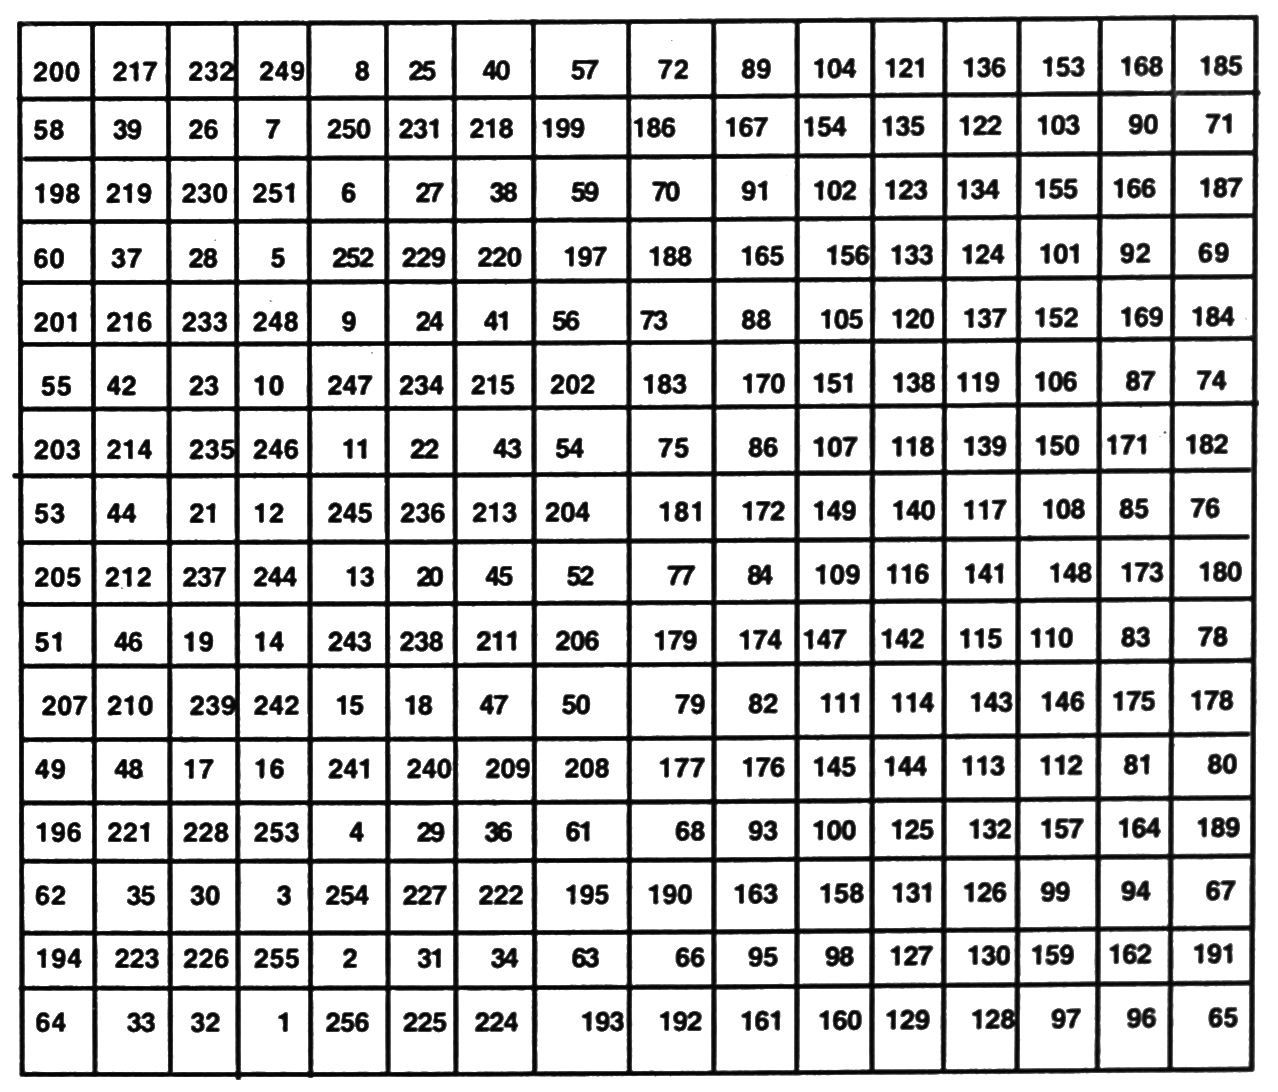
\includegraphics[scale=.9]{src/figures/chap7/fig7-7.jpg}
	\end{figure}
\end{itemize}

\section*{VIII. 4. ಮಾಯಾಚೌಕವೊಂದರ ವೈಚಿತ್ರ್ಯ}

ಮಾಯಾಚೌಕಗಳನ್ನು ಅಧ್ಯಯಿಸುವವರು ಅವುಗಳಲ್ಲಿನ ವೈವಿಧ್ಯತೆ, ವೈಶಿಷ್ಟ್ಯ ಮತ್ತು ವೈಚಿತ್ರ್ಯಗಳನ್ನು ಹೊರಹಾಕುವ ಕೆಲಸವನ್ನು ಮಾಡುತ್ತಲೇ ಇರುತ್ತಾರೆ. ಅವರು ಹೊರತಂದ ವಿಚಿತ್ರ ಫಲಗಳನ್ನು ನೋಡಿ ನಾವು ಆನಂದಿಸಬಹುದು. ತಾಳ್ಮೆ ಹಾಗೂ ಆಸಕ್ತಿ ಇದ್ದರೆ ನಾವು ಹೊಸತರ ಅನ್ವೇಷಣೆಯಲ್ಲಿ ತೊಡಗಬಹುದು.

ಒಂದು ವಿಶೇಷ ಮಾಯಾಚೌಕದ ವೈಚಿತ್ರ್ಯ ನೋಡೋಣ.

\begin{itemize}
	\item 1969 ನ್ನು 1ರಿಂದ 9ರವರೆಗಿನ ಸಂಖ್ಯೆಗಳಿಂದ ಗುಣಿಸಿ. ಗುಣಲಬ್ಧ ಹೀಗಿರುತ್ತದೆ.

	1969 3938 5907 7876 9845 11814 13783 15752 17721
	\item ಈ ಗುಣಲಬ್ಧಗಳನ್ನು 3 ಕ್ರಮವರ್ಗದ ಮಾಯಾಚೌಕವಾಗುವಂತೆ ಒಂದು ಮಾಯಾಚೌಕ ರಚಿಸಿ. ಸುಲಭವಾಗಿ ಅರ್ಥ ಮಾಡಿಕೊಳ್ಳಲು 1 ರಿಂದ 9 ವರೆಗಿನ ಸಂಖ್ಯೆಗಳ 3 ಕ್ರಮವರ್ಗದ ಚೌಕ ಕೊಟ್ಟಿದೆ. ಅದರ ಸಂಖ್ಯೆಗಳ ಸ್ಥಾನಗಳಲ್ಲಿ ಅವುಗಳಿಂದ 1969ನ್ನು ಗುಣಿಸಿದಾಗ ಬರುವ ಗುಣಲಬ್ಧ ಬರೆದಿದೆ. ಚಿತ್ರ ನೋಡಿ. A
	\begin{figure}[H]
<<<<<<< HEAD
	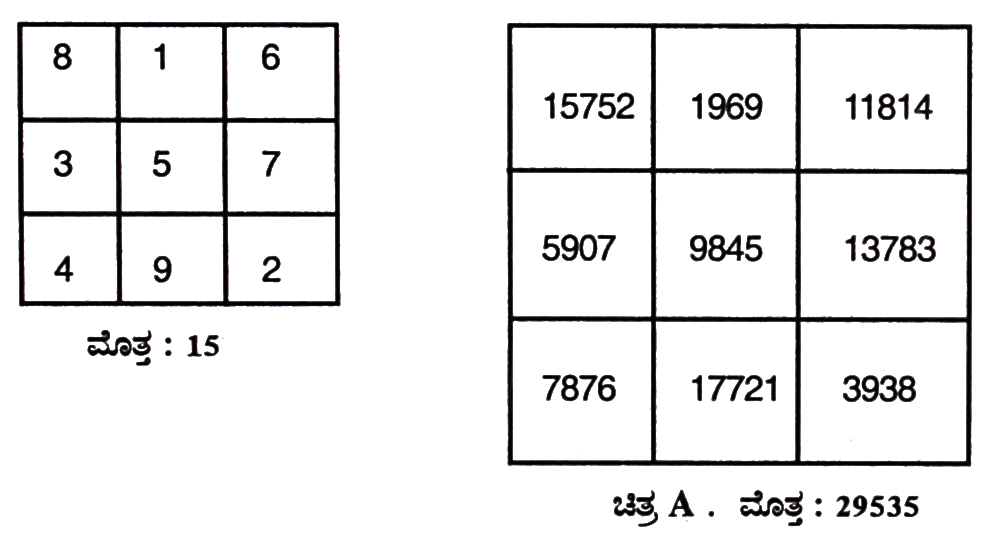
\includegraphics{src/figures/chap7/fig7-8.jpg}
=======
	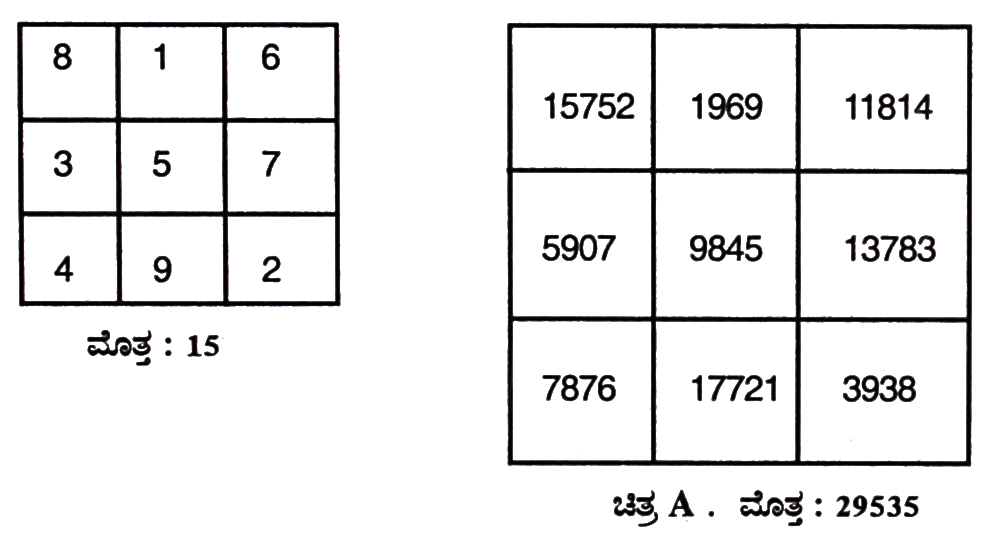
\includegraphics[scale=0.8]{src/figures/chap7/fig7.8.jpg}
>>>>>>> 6489d29d7c8981e9d16559f9e9427e431d3af0bd
	\end{figure}

	\item $A$ ಚೌಕದಲ್ಲಿನ ಪ್ರತಿ ಸಂಖ್ಯೆಯ ಏಕಸ್ಥಾನ (Unit Place)ದ ಅಂಕಿಯನ್ನು ವರ್ಜಿಸಿ, $3 \times 3$ ಚೌಕದಲ್ಲಿ $A^1$ ಬರೆಯಿರಿ.
	\begin{figure}[H]
<<<<<<< HEAD
	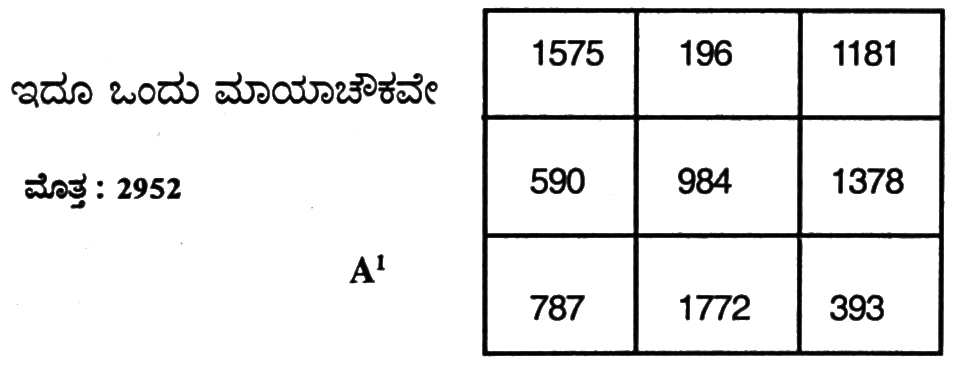
\includegraphics{src/figures/chap7/fig7-9.jpg}
=======
	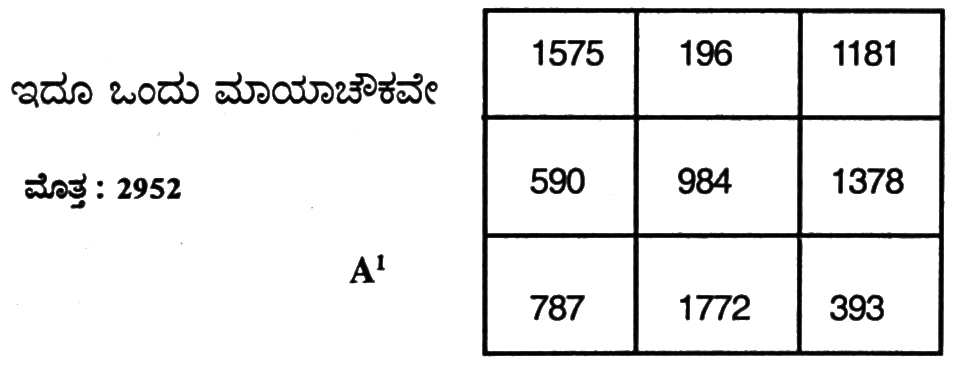
\includegraphics[scale=0.8]{src/figures/chap7/fig7.9.jpg}
>>>>>>> 6489d29d7c8981e9d16559f9e9427e431d3af0bd
	\end{figure}
\end{itemize}

ಈಗ A ಚೌಕದ ಸಂಖ್ಯೆಗಳಲ್ಲಿನ ಹತ್ತರ ಸ್ಥಾನದ (B), ನೂರರ ಸ್ಥಾನದ (C), ಸಾವಿರದ ಸ್ಥಾನದ (D), ಅಂಕಿಗಳನ್ನು ವರ್ಜಿಸಿ ಮಾಯಾಚೌಕಗಳನ್ನು ಬರೆದು ನೋಡೋಣ.
\begin{figure}[H]
<<<<<<< HEAD
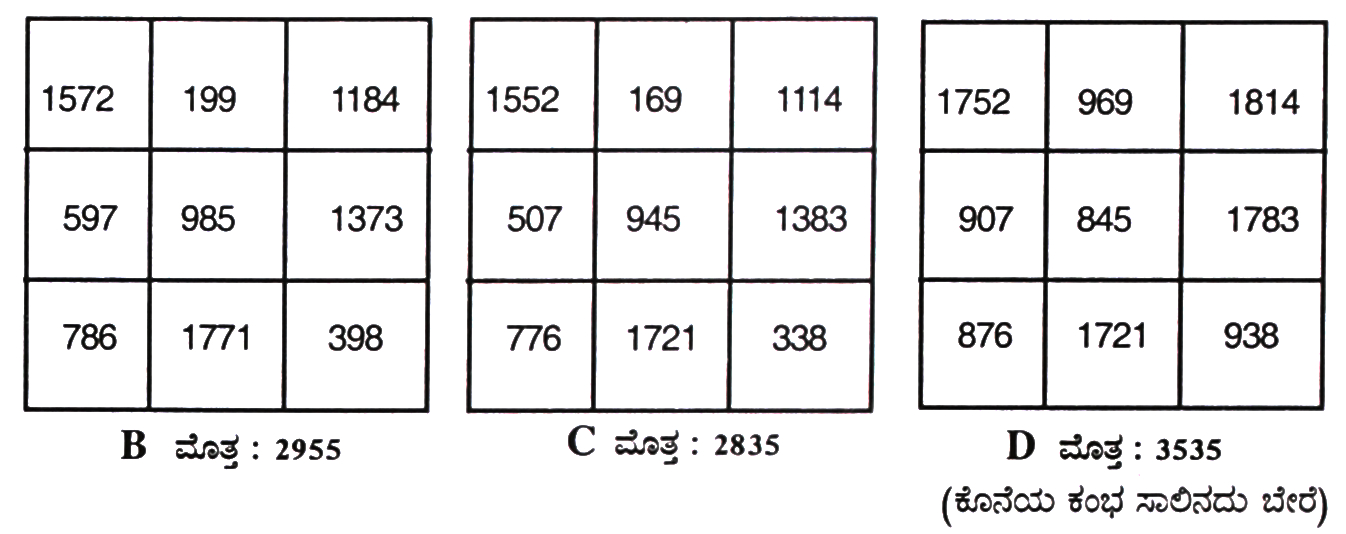
\includegraphics{src/figures/chap7/fig7-10.jpg}
=======
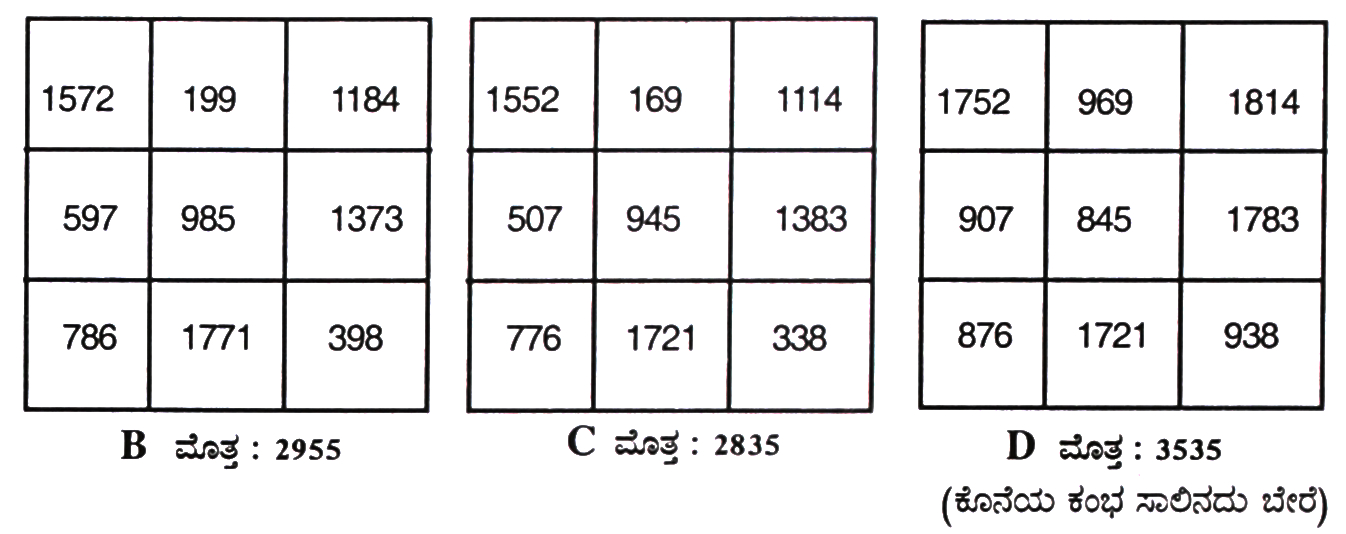
\includegraphics[scale=0.85]{src/figures/chap7/fig7.10.jpg}
>>>>>>> 6489d29d7c8981e9d16559f9e9427e431d3af0bd
\end{figure}

ಈ ಚೌಕಗಳ ಸಂಖ್ಯೆಗಳಲ್ಲಿನ ಏಕಸ್ಥಾನದ ಅಂಕಿ ವರ್ಜಿಸಿ ಮಾಯಾಚೌಕ ಬರೆಯೋಣ.
\begin{figure}[H]
<<<<<<< HEAD
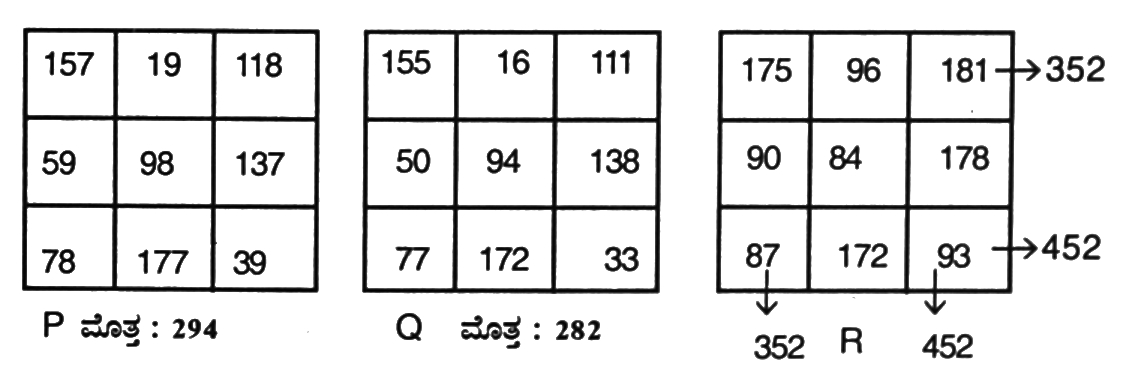
\includegraphics{src/figures/chap7/fig7-11.jpg}
=======
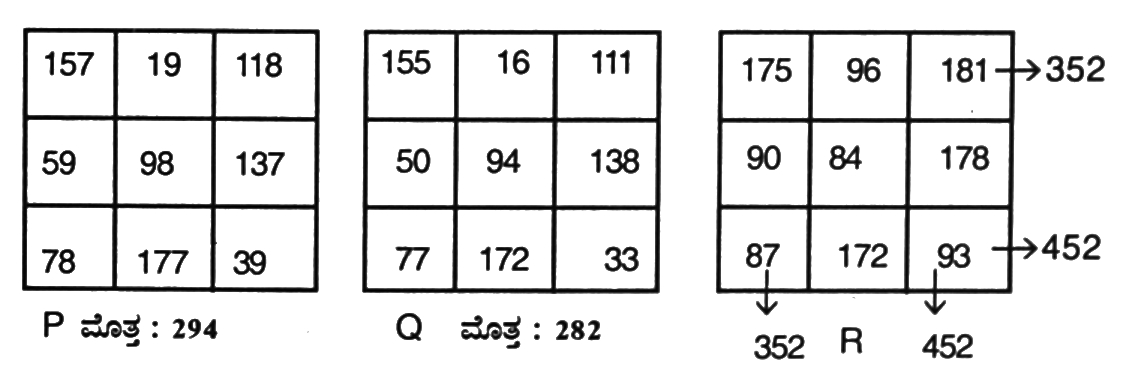
\includegraphics[scale=0.85]{src/figures/chap7/fig7.11.jpg}
>>>>>>> 6489d29d7c8981e9d16559f9e9427e431d3af0bd
\end{figure}

ಮೊದಲ ಎರಡೂ P ಮತ್ತು Q ಗಳು ಮಾಯಚೌಕಗಳೇ. R ಮಾತ್ರ ಊನ ಮಾಯಾಚೌಕ. ಇದರಲ್ಲಿ ಮೊದಲ ಅಡ್ಡಸಾಲು, ಕೊನೆಯ ಕಂಭಸಾಲುಗಳ ಮೊತ್ತ ಬೇರೆ. ಪುನಃ ಈ ಚೌಕಗಳಲ್ಲಿನ (P, Q, R) ಏಕಸ್ಥಾನದ ಅಂಕಿ ವರ್ಜಿಸಿ. ಚೌಕ ಬರೆಯಿರಿ. (P$^1$, Q$^1$, R$^1$ ಇರಲಿ)

ಮೊತ್ತ : 27
\begin{figure}[H]
<<<<<<< HEAD
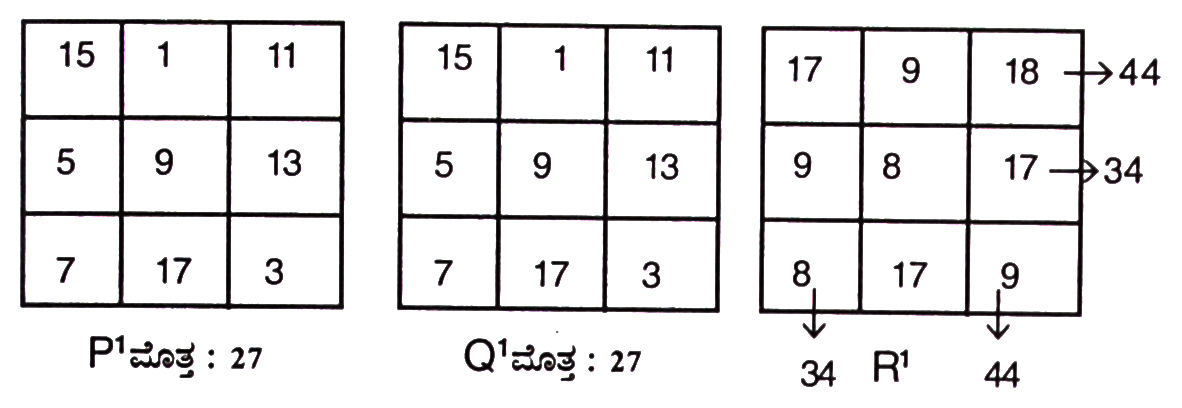
\includegraphics{src/figures/chap7/fig7-12.jpg}
=======
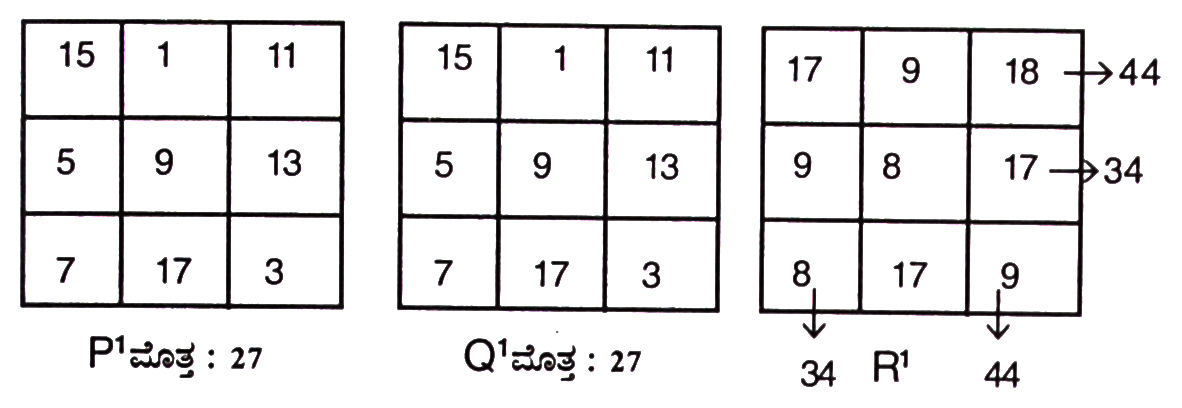
\includegraphics[scale=0.85]{src/figures/chap7/fig7.12.jpg}
>>>>>>> 6489d29d7c8981e9d16559f9e9427e431d3af0bd
\end{figure}

ಇವುಗಳಲ್ಲಿ P ಮತ್ತು Q ಚೌಕಗಳಿಂದ ಮಾಯಾಚೌಕ ಲಭಿಸುತ್ತದೆ. R ಚೌಕದಿಂದ ಮತ್ತೆ ಊನ ಮಾಯಾಚೌಕ ದೊರಕಿದೆ. ಇದರ ಎರಡು ಸಾಲು ಬಿಟ್ಟರೆ ಉಳಿದ ಸಾಲುಗಳ (ಕರ್ಣ\-ಗಳನ್ನು ಒಳಗೊಂಡಂತೆ) ಮೊತ್ತ 34.

ಈ ಚೌಕಗಳ ವೈಚಿತ್ರ್ಯ ಇಷ್ಟೇ ಅಲ್ಲ. ಇವುಗಳಲ್ಲಿ ಇನ್ನೊಂದು ರೀತಿಯ ಪ್ರಕ್ರಿಯೆಯನ್ನು ಪ್ರಯತ್ನಿಸೋಣ. ಏಕಸ್ಥಾನದ ಅಂಕಿಯನ್ನು ವರ್ಜಿಸಿ, ಹತ್ತರ, ಸ್ಥಾನದ ಅಂಕಿಗೆ ಅದರ ಹಿಂದಿನ ಸ್ಥಾನದ ಸಂಖ್ಯೆ ಆದೇಶಿಸಿ.

ಉದಾ : ಏಕಸ್ಥಾನ ಅಂಕಿ ಬಿಟ್ಟಾಗ 1575 (15752ರಲ್ಲಿ 2 ಬಿಟ್ಟಿದೆ) A ಚೌಕದಲ್ಲಿ

ಇದರಲ್ಲಿ ಏಕಸ್ಥಾನದ ಅಂಕಿ ಬಿಟ್ಟಾಗ 157 (5ನ್ನು ಬಿಟ್ಟಿದೆ) $A^1$ ಚೌಕದಲ್ಲಿ

\begin{tabular}{ll}
ಹತ್ತರಸ್ಥಾನದ ಅಂಕಿ 7. ಇದರ ಹಿಂದಿನ ಸಂಖ್ಯೆ 15. & \multirow{3}{2cm}{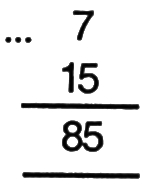
\includegraphics[scale=.8]{src/figures/chap7/fig7-33.jpg}}\\
ಇದನ್ನು ಆದೇಶಿಸಿದಾಗ ... & \\
ಇದೇ ರೀತಿ ಉಳಿದ ಸಂಖ್ಯೆಗಳಲ್ಲೂ ಮಾಡಿದೆ.
\end{tabular}

\begin{figure}[H]
<<<<<<< HEAD
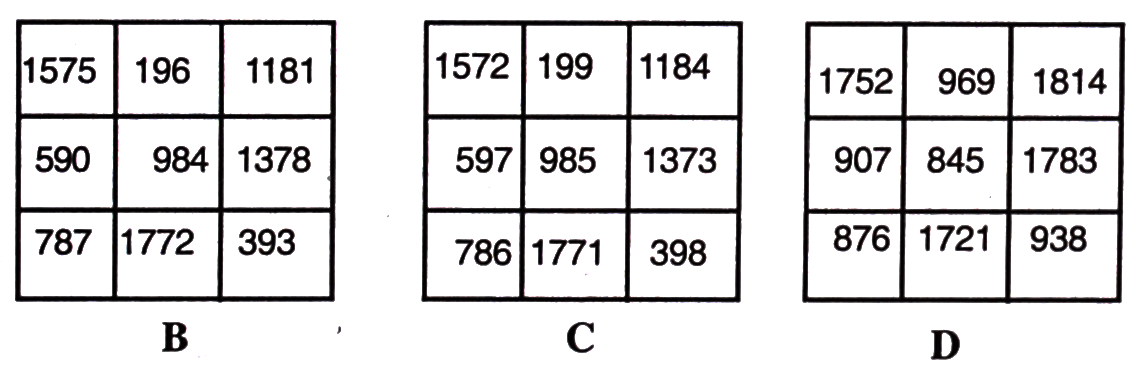
\includegraphics{src/figures/chap7/fig7-13.jpg}
=======
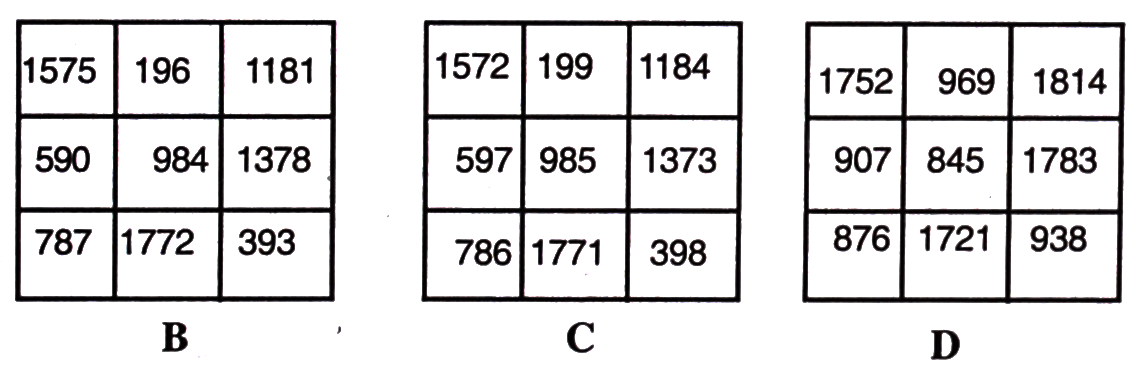
\includegraphics[scale=0.85]{src/figures/chap7/fig7.13.jpg}
>>>>>>> 6489d29d7c8981e9d16559f9e9427e431d3af0bd
\end{figure}

ಇವುಗಳಲ್ಲಿ ಏಕಸ್ಥಾನದ ಅಂಕಿ ಬಿಟ್ಟು , ಹಿಂದಿನ ಸಂಖ್ಯೆ ಮುಂದಕ್ಕೆ ಆದೇಶಿಸಿ.
\begin{figure}[H]
<<<<<<< HEAD
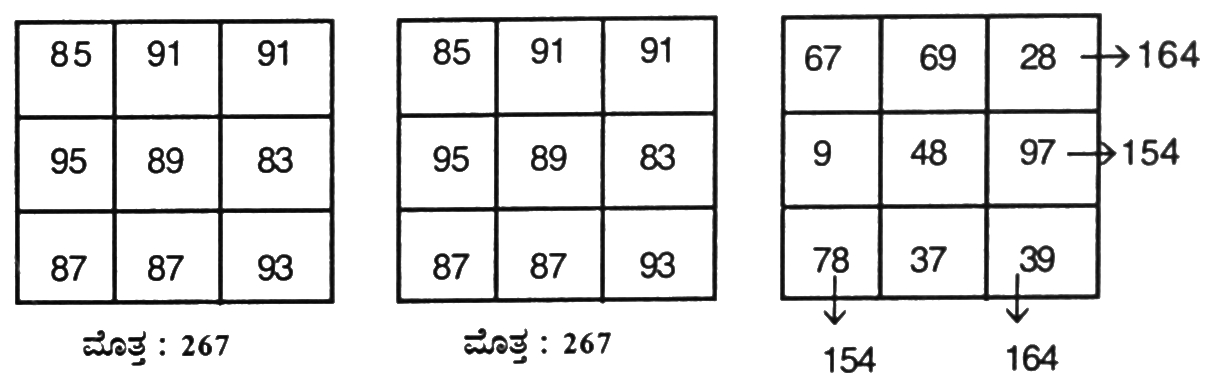
\includegraphics{src/figures/chap7/fig7-14.jpg}
=======
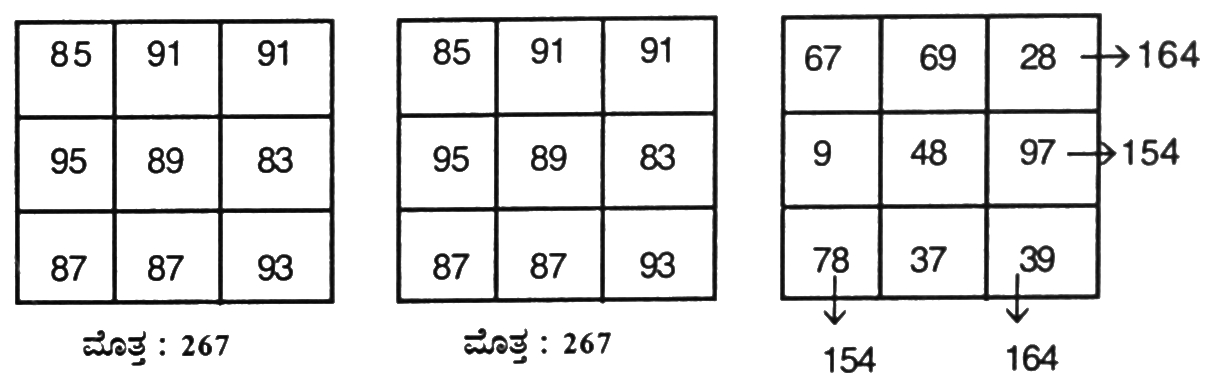
\includegraphics[scale=0.85]{src/figures/chap7/fig7.14.jpg}
>>>>>>> 6489d29d7c8981e9d16559f9e9427e431d3af0bd
\end{figure}

A ಚೌಕದಲ್ಲಿನ ಸಂಖ್ಯೆಗಳಲ್ಲಿ ಏಕಸ್ಥಾನದ ಅಂಕಿ ಬಿಟ್ಟು ಹಿಂದಿನ ಸಂಖ್ಯೆಯನ್ನು ಮುಂದಕ್ಕೆ ಆದೇಶಿಸಿದಾಗಲೂ ಮಾಯಾಚೌಕ ಲಭ್ಯ . ಮೊತ್ತ : 2547
\begin{figure}[H]
<<<<<<< HEAD
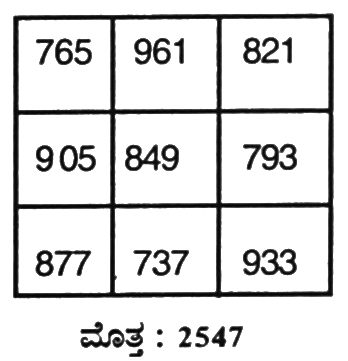
\includegraphics{src/figures/chap7/fig7-15.jpg}
=======
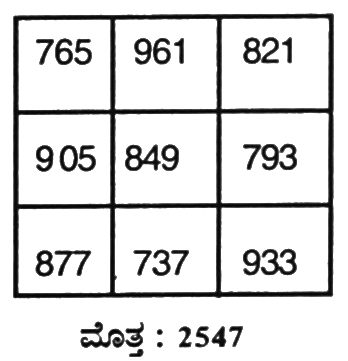
\includegraphics[scale=0.85]{src/figures/chap7/fig7.15.jpg}
>>>>>>> 6489d29d7c8981e9d16559f9e9427e431d3af0bd
\end{figure}

ಹೇಗಿದೆ ನೋಡಿ ಮಾಯಾಚೌಕಗಳ ಕರಾಮತ್ತು. ಇವುಗಳನ್ನು ಪ್ರಸ್ತುತಪಡಿಸಿದ ಗಣಿತಜ್ಞರಿಗೆ ನಮೋ ನಮಃ

\textbf{VIII. 5.} ಒಂದು ಮಾಯಾಚೌಕದ ಸಂಖ್ಯೆಗಳ ವರ್ಗಗಳನ್ನು (Squares) ಅನುರೂಪ ಮನೆಗಳಲ್ಲಿ ತುಂಬಿಸಿದಾಗ ಮತ್ತೊಂದು ಮಾಯಾಚೌಕ ಲಭಿಸಬೇಕೆಂದಿಲ್ಲ. 1 ರಿಂದ 9 ರವರೆ\-ಗಿನ ಸಂಖ್ಯೆಗಳನ್ನು ಬಳಸಿ 3 ಕ್ರಮವರ್ಗದ ಮಾಯಾಚೌಕ ರಚಿಸೋಣ. ಮತ್ತೊಂದು $3 \times 3$ಚೌಕದಲ್ಲಿ ಈ ಸಂಖ್ಯೆಗಳ ವರ್ಗ (Square) ಸಂಖ್ಯೆಗಳನ್ನು ಬರೆದು, ಅದು ಮಾಯಾಚೌಕವೇ ಪರೀಕ್ಷಿಸೋಣ.
\begin{figure}[H]
<<<<<<< HEAD
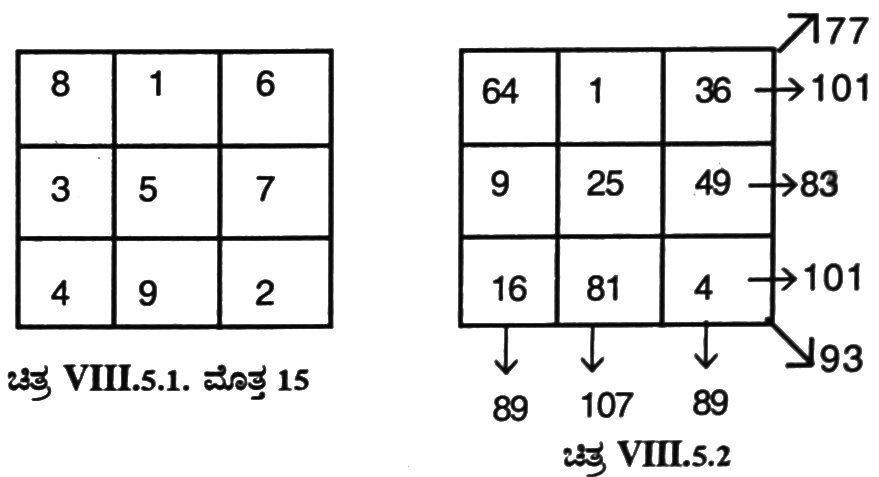
\includegraphics{src/figures/chap7/fig7-16.jpg}
=======
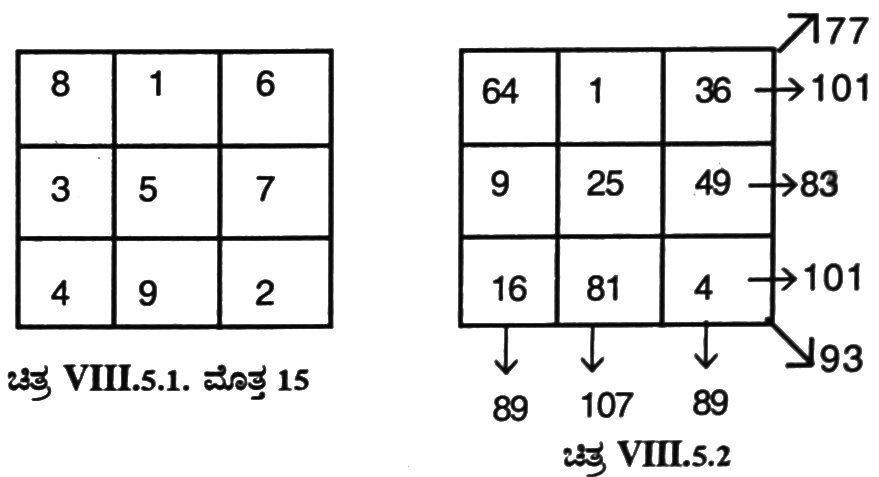
\includegraphics[scale=0.85]{src/figures/chap7/fig7.16.jpg}
>>>>>>> 6489d29d7c8981e9d16559f9e9427e431d3af0bd
\end{figure}

ಚಿತ್ರ VIII. 5.2. ರಲ್ಲಿರುವ ಚೌಕದ ಅಡ್ಡಸಾಲು, ಕಂಭಸಾಲು ಮತ್ತು ಕರ್ಣಗಳ ಸಂಖ್ಯೆಗಳ ಮೊತ್ತ ಬರೆದಿದೆ. ಇದು ಮಾಯಾಚೌಕವಲ್ಲ ಎನ್ನುವುದು ವೇದ್ಯ.

ಈ ಕೆಳಗಿನ ಮಾಯಾಚೌಕಗಳನ್ನು ಗಮನಿಸಿ.
\begin{figure}[H]
<<<<<<< HEAD
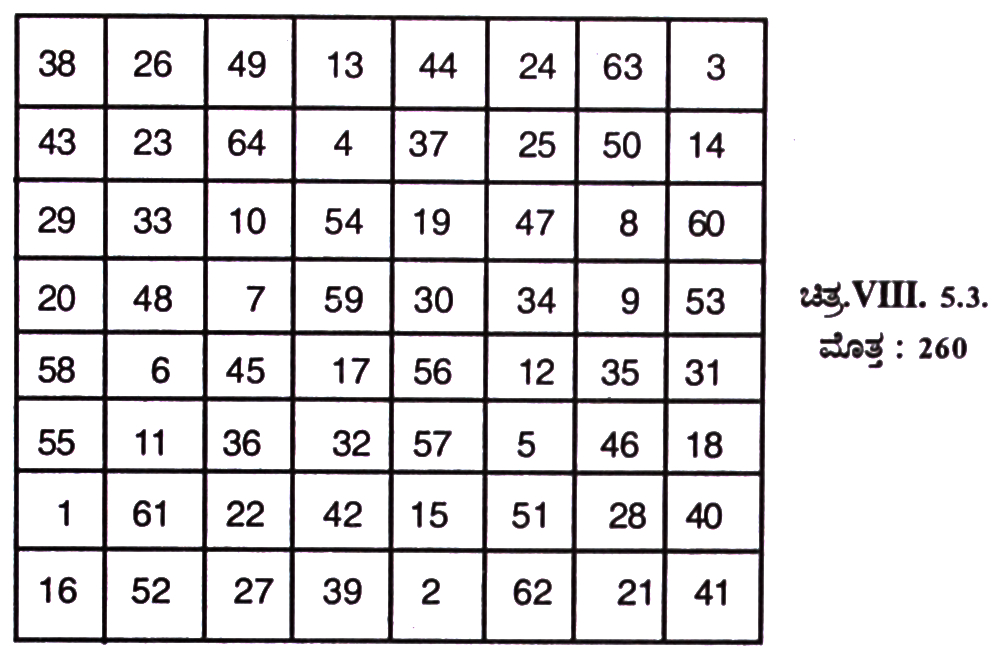
\includegraphics{src/figures/chap7/fig7-17.jpg}
=======
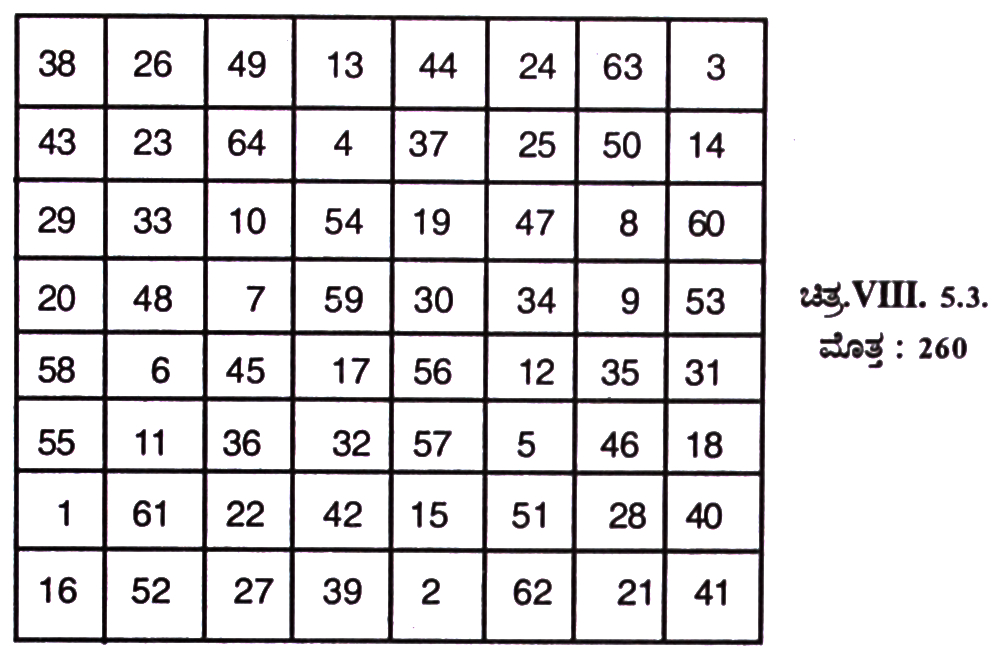
\includegraphics[scale=0.85]{src/figures/chap7/fig7.17.jpg}
>>>>>>> 6489d29d7c8981e9d16559f9e9427e431d3af0bd
\end{figure}

ಚಿತ್ರ. VIII.5.3 ಚೌಕದ ಸಂಖ್ಯೆಗಳ ವರ್ಗ ಸಂಖ್ಯೆಗಳನ್ನು ಅನುರೂಪ ಮನೆಗಳಲ್ಲಿ ತುಂಬಿ\-ಸಿದೆ.
\begin{figure}[H]
<<<<<<< HEAD
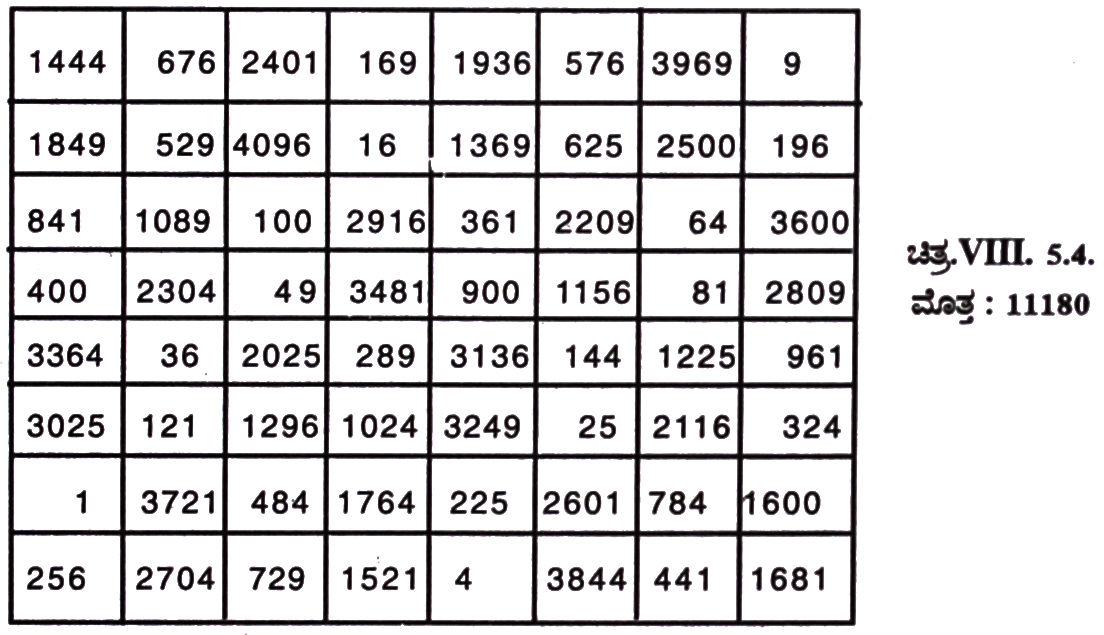
\includegraphics{src/figures/chap7/fig7-18.jpg}
=======
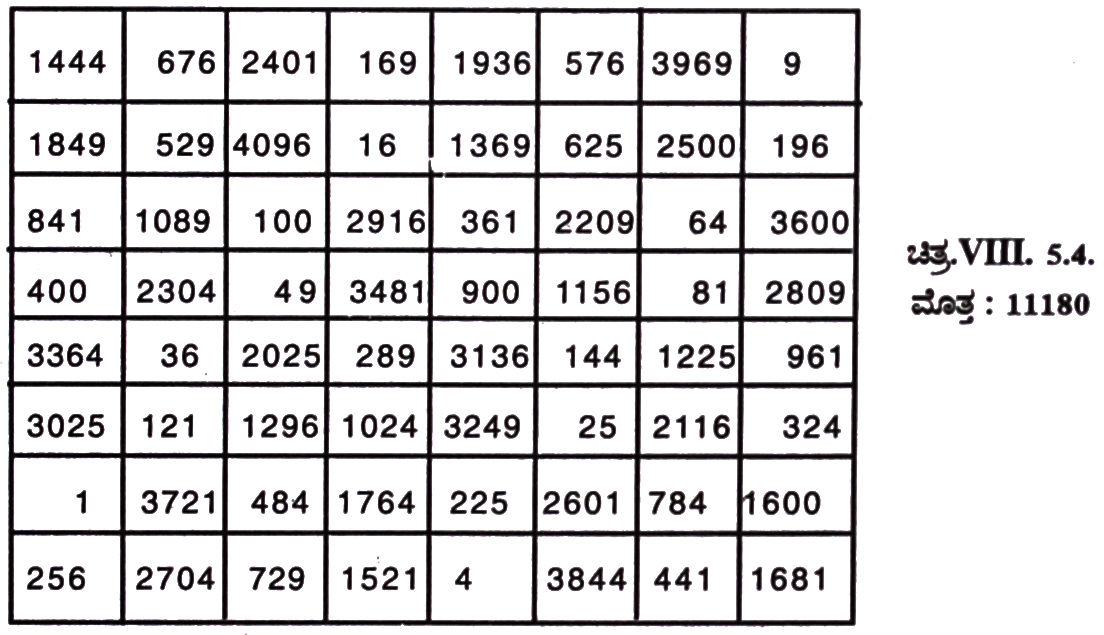
\includegraphics[scale=0.85]{src/figures/chap7/fig7.18.jpg}
>>>>>>> 6489d29d7c8981e9d16559f9e9427e431d3af0bd
\end{figure}

ಚಿತ್ರ.VIII.5.3 ರಲ್ಲಿರುವುದು 8 ಕ್ರಮವರ್ಗದ ಮಾಯಾಚೌಕ. 1ರಿಂದ 64 ವರೆಗಿನ ಕ್ರಮಾಗತ ಸಂಖ್ಯೆಗಳಿಂದಾಗಿದೆ. ಮೊತ್ತ 260

ಚಿತ್ರ.VIII.5.4 ರಲ್ಲಿರುವುದೂ 8 ಕ್ರಮವರ್ಗದ ಮಾಯಾಚೌಕವೇ. ಇದರಲ್ಲಿ ಚಿತ್ರ.VIII.5.3 ರಲ್ಲಿನ ಸಂಖ್ಯೆಗಳನ್ನು ವರ್ಗಮಾಡಿ (Square) ಅನುರೂಪ ಮನೆಗಳಲ್ಲಿ ತುಂಬಿಸಿದೆ. ಇದರ ಮೊತ್ತ 11180

ಈ ಮಾಯಾಚೌಕದ ವೈಶಿಷ್ಟ್ಯ ಇಷ್ಟೇ ಅಲ್ಲ. ಚಿತ್ರ VIII. 5.3ರಲ್ಲಿರುವ ಮಾಯಾಚೌಕದ ಸಂಖ್ಯೆಗಳನ್ನು ಪ್ರತಿಯೊಂದನ್ನೂ 65 ರಿಂದ ಕಳೆದು, ಬರುವ ಸಂಖ್ಯೆಗಳನ್ನು ಅದೇ ಮನೆಗಳಲ್ಲಿ ತುಂಬಿಸಿದರೆ ಮತ್ತೊಂದು ಮಾಯಾಚೌಕ ಸಿದ್ಧಿಸುತ್ತದೆ. ಚಿತ್ರ VIII. 5.5 ನೋಡಿ. ಇದರ ಮೊತ್ತವೂ 260. ಹೀಗೆ ಲಭಿಸಿದ ಮಾಯಾಚೌಕದ ಸಂಖ್ಯೆಗಳ ವರ್ಗಗಳನ್ನು ಅನುರೂಪ ಮನೆಗಳಲ್ಲಿ ಬರೆದರೆ ಮತ್ತೊಂದು ಮಾಯಾಚೌಕ ಸಿದ್ಧಿಸುತ್ತದೆ. ಮೊತ್ತ 11180. ಈ ಕೆಳಗಿನ ಚಿತ್ರಗಳನ್ನು ನೋಡಿ VIII. 5.6
\begin{figure}[H]
<<<<<<< HEAD
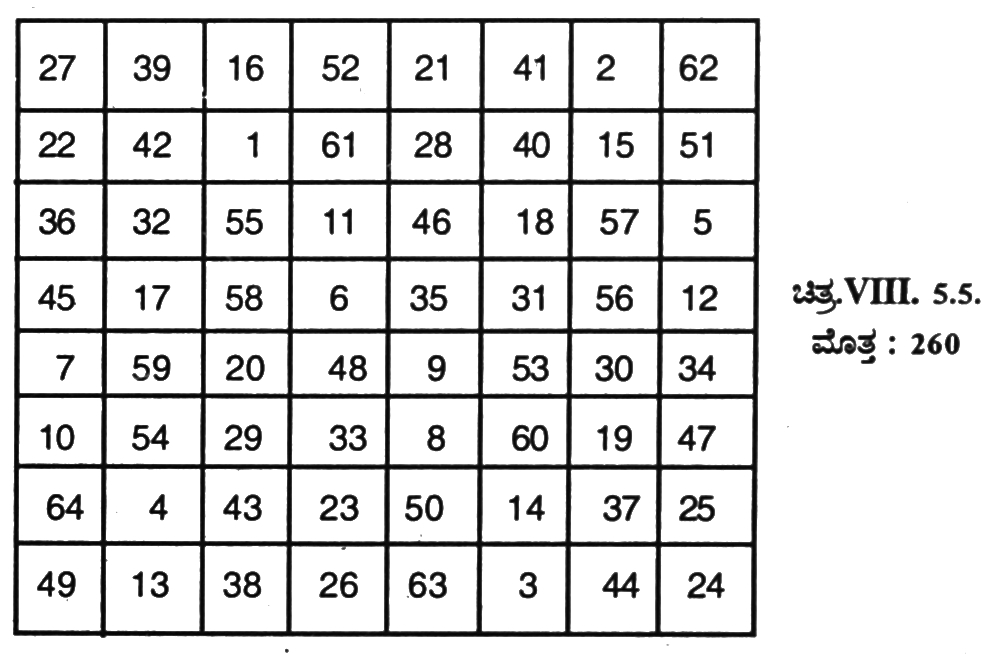
\includegraphics{src/figures/chap7/fig7-19.jpg}
\end{figure}
\begin{figure}[H]
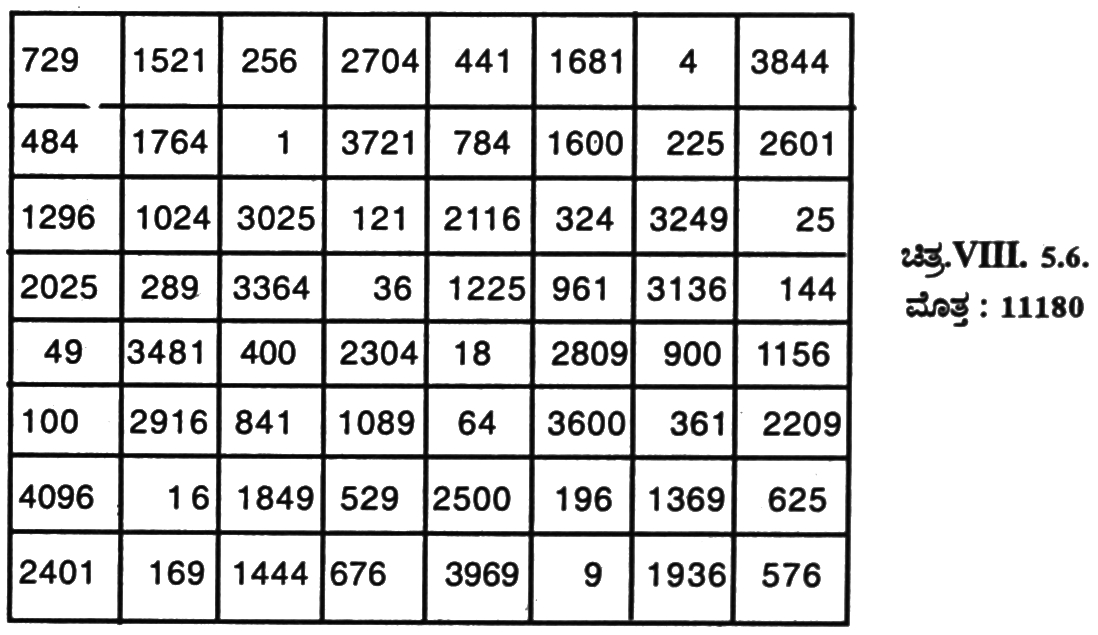
\includegraphics{src/figures/chap7/fig7-20.jpg}
=======
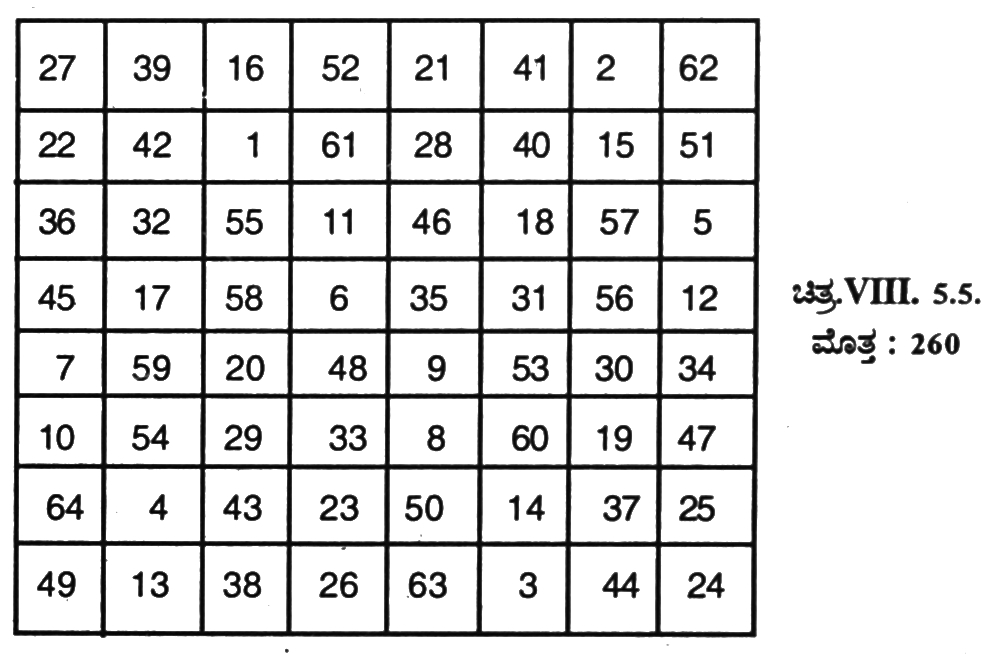
\includegraphics[scale=0.85]{src/figures/chap7/fig7.19.jpg}
\end{figure}
\begin{figure}[H]
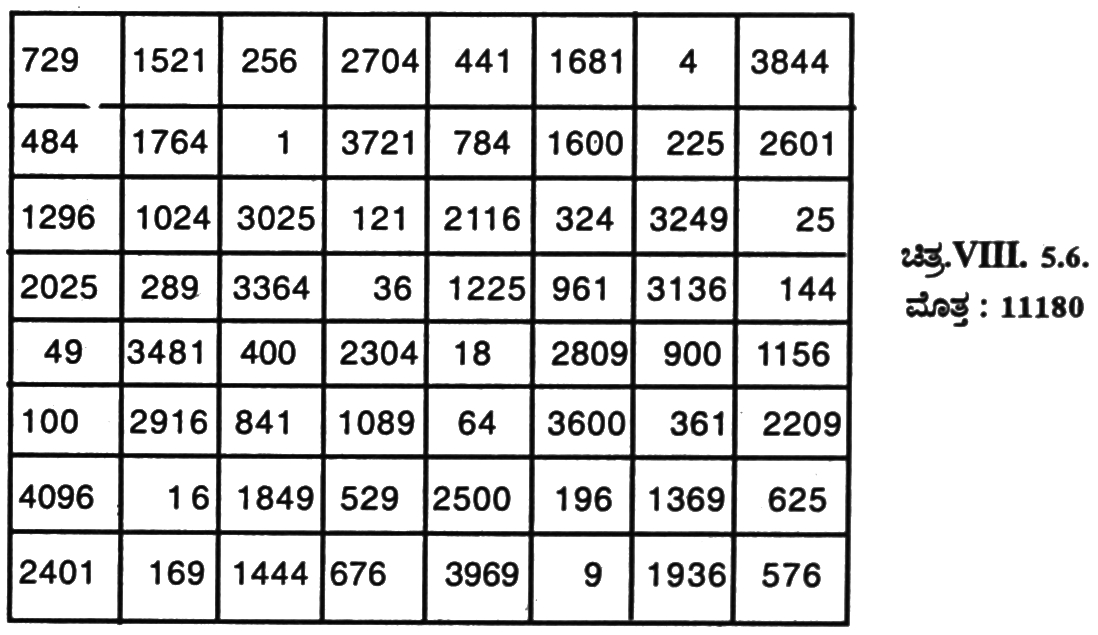
\includegraphics[scale=0.85]{src/figures/chap7/fig7.20.jpg}
>>>>>>> 6489d29d7c8981e9d16559f9e9427e431d3af0bd
\end{figure}

ಚಿತ್ರ VIII.5.5.ರ ಚೌಕದ ಸಂಖ್ಯೆಗಳ ವರ್ಗಗಳಿಂದಾದುದು.

ಹೇಗಿದೆ ನೋಡಿ ಗಣಿತಜ್ಞರ ಸೃಜನಶೀಲತೆ

\section*{VIII. 6. ಅಕ್ಷರ ಸಂಖ್ಯಾ ಮಾಯಾಚೌಕ (Alphamagaic Square)}

ಮಾಯಾಚೌಕಗಳನ್ನು ಅಭ್ಯಸಿಸುವ ಕೆಲವರಿಗೆ ಹೊಸ ಬಗೆಯ ಮಾಯಾಚೌಕ ರಚಿಸಬೇಕೆಂಬ ಹಂಬಲ ಇರುವುದು ಸಹಜ. ಹಲವಾರು ಪ್ರಯತ್ನಗಳಲ್ಲಿ ಒಮ್ಮೊಮ್ಮೆ ಯಶಸ್ಸು ಸಿಗುವುದೂ ಉಂಟು. ಇಂತಹ ಒಂದು ವಿಶಿಷ್ಟವಾದ ಮಾಯಾಚೌಕ ಇಲ್ಲಿದೆ. ಇದು 3 ಕ್ರಮವರ್ಗದ\break ಮಾಯಾಚೌಕ. ಮೊತ್ತ 45
\begin{figure}[H]
<<<<<<< HEAD
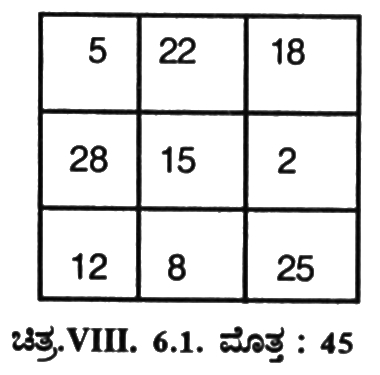
\includegraphics{src/figures/chap7/fig7-21.jpg}
=======
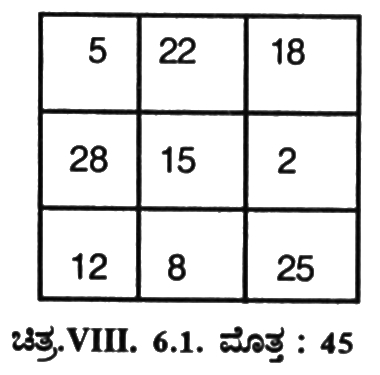
\includegraphics[scale=0.8]{src/figures/chap7/fig7.21.jpg}
>>>>>>> 6489d29d7c8981e9d16559f9e9427e431d3af0bd
\end{figure}

ಈ ಮಾಯಾಚೌಕದ ಸಂಖ್ಯೆಗಳನ್ನು ಇಂಗ್ಲೀಷ್ ಅಕ್ಷರಗಳಲ್ಲಿ ಒಂದು $3 \times 3$ಚೌಕದಲ್ಲಿ, ಅನುರೂಪ ಮನೆಗಳಲ್ಲಿ ಬರೆಯೋಣ.

ಇದನ್ನು \textbf{ಲೀ ಸ್ವಾಲೋಸ್} ಎಂಬಾತ 1986ರಲ್ಲಿ ರಚಿಸಿದ.

\newpage

\begin{figure}[H]
<<<<<<< HEAD
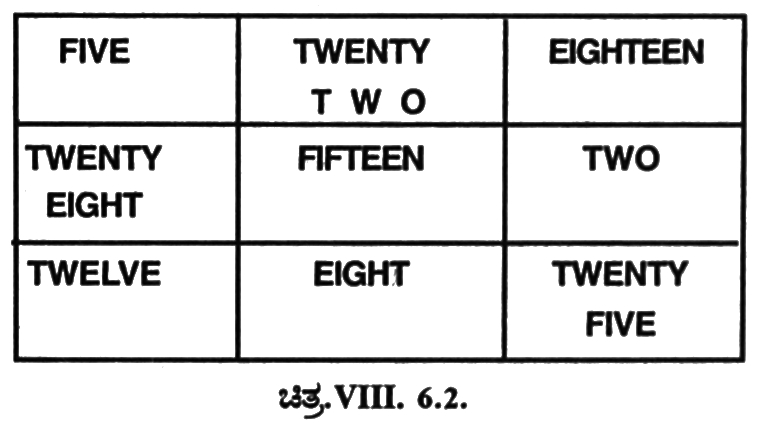
\includegraphics{src/figures/chap7/fig7-22.jpg}
=======
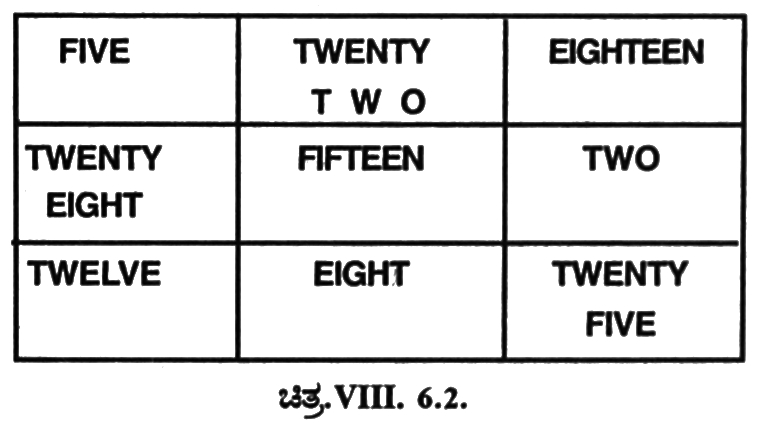
\includegraphics[scale=0.8]{src/figures/chap7/fig7.22.jpg}
>>>>>>> 6489d29d7c8981e9d16559f9e9427e431d3af0bd
\end{figure}

ಈ ಚೌಕದ ಪದಗಳಲ್ಲಿರುವ ಅಕ್ಷರಗಳನ್ನು ಎಣಿಸಿ, $3 \times 3$ಚೌಕದಲ್ಲಿ ಅನುರೂಪ ಮನೆ\-ಗಳಲ್ಲಿ ಬರೆಯೋಣ. (FIVE - 4 ನಾಲ್ಕು ಅಕ್ಷರಗಳಿವೆ)
\begin{figure}[H]
<<<<<<< HEAD
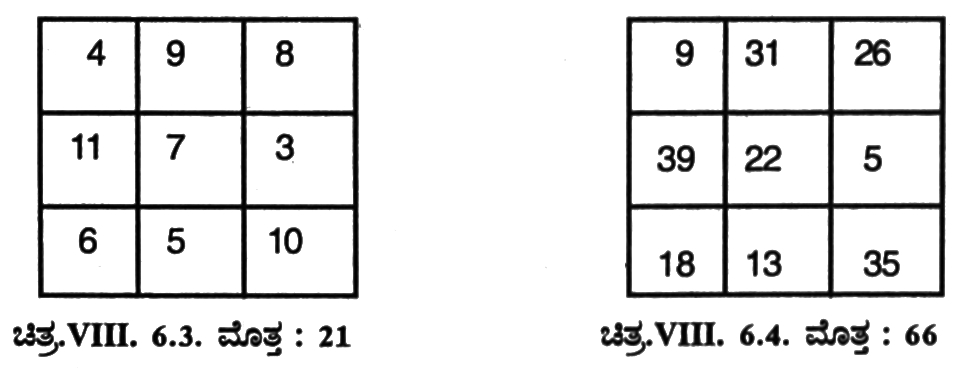
\includegraphics{src/figures/chap7/fig7-23.jpg}
=======
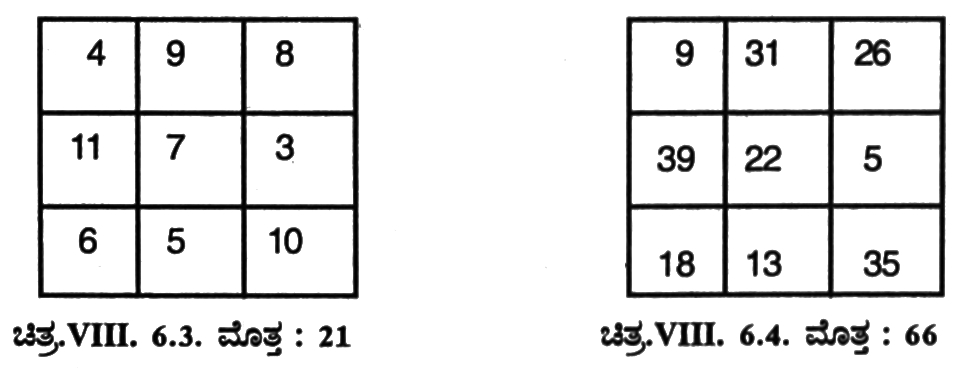
\includegraphics[scale=0.8]{src/figures/chap7/fig7.23.jpg}
>>>>>>> 6489d29d7c8981e9d16559f9e9427e431d3af0bd
\end{figure}

ಇದೂ ಒಂದು ಮಾಯಾಚೌಕವೇ. ಇಂತಹವು ಅತಿ ವಿರಳ. ಖುಷಿಗಾಗಿ ಕೆಲವರು ಇಂತಹ\-ವನ್ನು ರಚಿಸಿದ್ದಾರೆ. ನಾವು ನೋಡಿ ಸಂತೋಷಪಡಬಹುದು. ಚಿತ್ರ VIII. 6.1. ಮತ್ತು ಚಿತ್ರ VIII. 6.3 ರಲ್ಲಿ ಮಾಯಾಚೌಕದ ಅನುರೂಪ ಸಂಖ್ಯೆಗಳನ್ನು ಕೂಡಿಸಿ. ಮತ್ತೊಂದು $3 \times 3$ ಚೌಕದಲ್ಲಿ ಬರೆಯಿರಿ. ಅದೂ ಒಂದು ಮಾಯಾಚೌಕವೇ ಮೊತ್ತ 66. (VIII. 6.4)

\section*{ಅನ್ಯ ಪ್ರಕ್ರಿಯೆ ಮಾಯಾಚೌಕಗಳು}

ಸಾಮಾನ್ಯವಾಗಿ ಮಾಯಾಚೌಕಗಳಲ್ಲಿ ಅಡ್ಡಸಾಲು, ಕಂಭಸಾಲು ಮತ್ತು ಕರ್ಣಗಳಲ್ಲಿನ ಸಂಖ್ಯೆ\-ಗಳ ಮೊತ್ತ ಸ್ಥಿರಾಂಕವಾಗಬೇಕೆಂಬುದು ನಿಯಮ. ಆದರೆ ಈಚೆಗೆ ಹಲವು ಗಣಿತಾಸಕ್ತರು\break ಸಾಲುಗಳ ಸಂಖ್ಯೆಗಳ ಮೊತ್ತದ ಬದಲಾಗಿ ಗಣಿತದ ಬೇರೆ ಪ್ರಕ್ರಿಯೆಗಳನ್ನು ಅಂದರೆ ವ್ಯವಕಲನ, ಗುಣಾಕಾರ ಮತ್ತು ಭಾಗಾಕಾರಗಳನ್ನು ಅನ್ವಯಿಸಿ ನಿಶ್ಚಿತ ಲಬ್ಧ ಬರುವಂತೆ ಚೌಕಗಳನ್ನು ರಚಿಸಿ\-ದ್ದಾರೆ. ಇವುಗಳನ್ನು ನೋಡಿದಾಗ ಮಾಯಾಚೌಕಗಳ ಹರವನ್ನು ಮತ್ತಷ್ಟು ಹಿಗ್ಗಿಸ\-ಬಹುದು ಎನಿಸು\-ತ್ತದೆ.

\section*{ III. 7. ವ್ಯವಕಲನ ಮಾಯಾಚೌಕ}

ವ್ಯವಕಲನವೆಂದರೆ ಒಂದು ಸಂಖ್ಯೆಯಿಂದ ಮತ್ತೊಂದು ಸಂಖ್ಯೆಯನ್ನು ಕಳೆಯುವುದು. ಮಾಯಾ\-ಚೌಕದಲ್ಲಿ ಕಳೆಯಲು ಒಂದು ನಿಯಮವಿದೆ. ಅಡ್ಡಸಾಲು, ಕಂಭಸಾಲು, ಅಥವಾ ಕರ್ಣಗಳ ಸಂಖ್ಯೆ ತೆಗೆದುಕೊಳ್ಳಿ. ಯಾವುದೇ ಸಾಲಿನ ಎರಡನೆ ಸಂಖ್ಯೆಯಿಂದ ಮೊದಲ ಸಂಖ್ಯೆ ಕಳೆಯಿರಿ. ಬಂದ ಉತ್ತರವನ್ನು ಅದೇಸಾಲಿನ ಮೂರನೆ ಸಂಖ್ಯೆಯಿಂದ ಕಳೆಯಿರಿ. ಆ ಸಾಲಿನ\break ಕೊನೆಯ ಸಂಖ್ಯೆವರೆಗೂ ಮುಂದುವರಿಸಿ. ಅಂತಿಮವಾಗಿ ಒಂದು ಉತ್ತರ ಸಿಕ್ಕುತ್ತದೆ.\break ಯಾವುದೇ ಸಾಲಿನ ಸಂಖ್ಯೆಗಳನ್ನು ಈ ಪ್ರಕ್ರಿಯೆಗೆ ಒಳಪಡಿಸಿದಾಗಲೂ ಉತ್ತರವು ಅದೇ ಇರುತ್ತದೆ. ಕಳೆಯುವಾಗ ಕೆಲವೊಮ್ಮೆ ಋಣ ಸಂಖ್ಯೆಗಳು ಬರಬಹುದು. ಆಗ ಅದನ್ನು ಮುಂದಿನ ಸಂಖ್ಯೆ ಕಳೆಯುವಾಗ ಎಚ್ಚರವಿರಲಿ.
\begin{figure}[H]
<<<<<<< HEAD
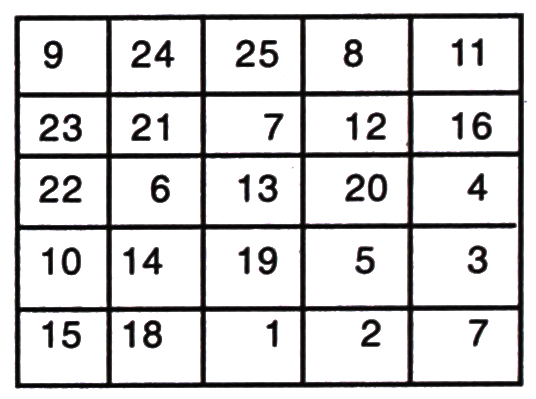
\includegraphics{src/figures/chap7/fig7-24.jpg}
=======
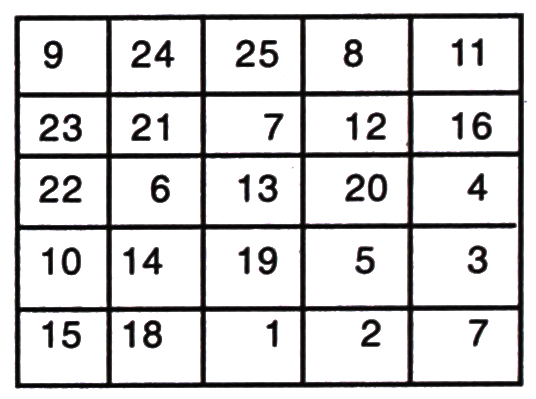
\includegraphics[scale=0.8]{src/figures/chap7/fig7.24.jpg}
>>>>>>> 6489d29d7c8981e9d16559f9e9427e431d3af0bd
\end{figure}

ಉದಾಹರಣೆಗೆ :
\begin{itemize}
	\item 5 ಕ್ರಮವರ್ಗದ ಚೌಕ
	\item 1ರಿಂದ 25 ವರೆಗೆ ಕ್ರಮಾಗತ ಸಂಖ್ಯೆಗಳನ್ನು ಬಳಸಿದೆ
	\item ಪ್ರಕ್ರಿಯೆ
\end{itemize}

1ನೇ ಅಡ್ಡಸಾಲು :

$24-9=15; 25-15=10; 8-10=-2; 11-(-2)-= \boxed{13}$

1ನೇ ಕಂಭಸಾಲು :

$23-9=14; 22-14=8; 10-8=2; 15-2= \boxed{13}$

ಒಂದು ಕರ್ಣ :

$14-15=-1; 13-(-1)=14; 12-14=-2; 11-(-1)-= \boxed{13}$

ಉಳಿದ ಸಾಲುಗಳ ಸಂಖ್ಯೆಗಳಿಗೂ ಈ ಪ್ರಕ್ರಿಯೆ ಅನ್ವಯಿಸಿ ಪ್ರಮಾಣಿಸಬಹುದು.
\begin{center}
*****
\end{center}
\begin{figure}[H]
<<<<<<< HEAD
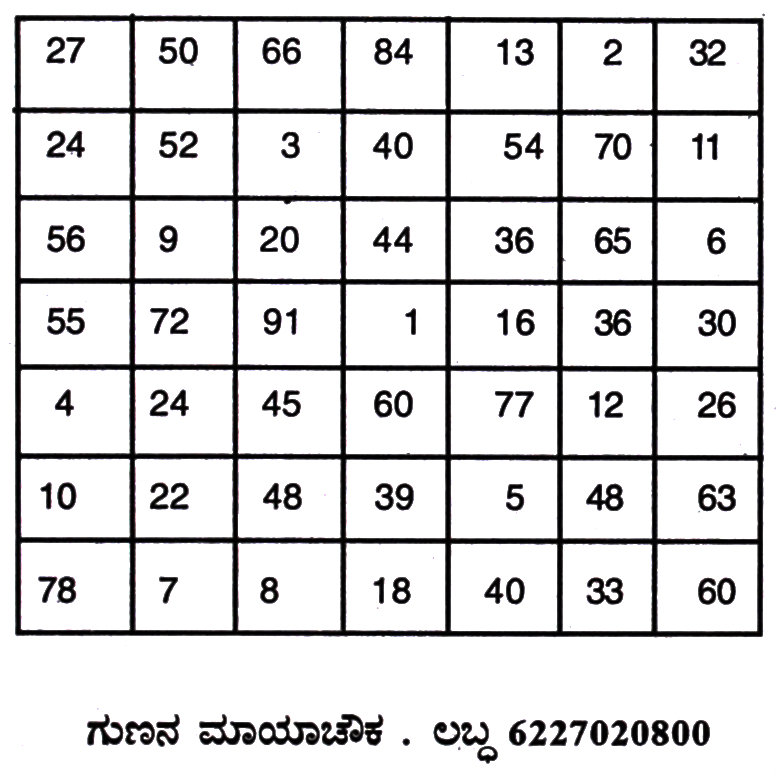
\includegraphics{src/figures/chap7/fig7-25.jpg}
=======
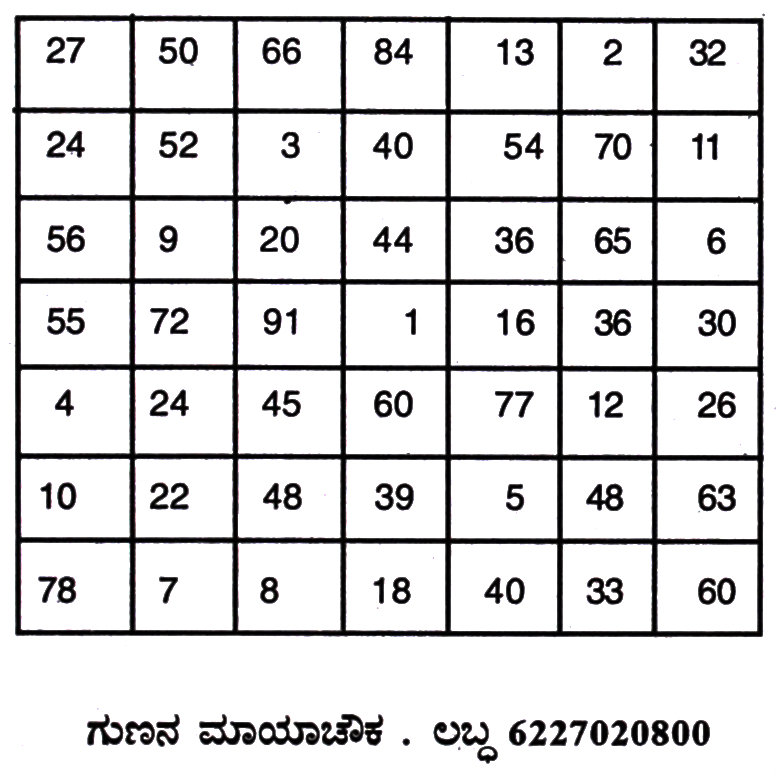
\includegraphics[scale=0.8]{src/figures/chap7/fig7.25.jpg}
>>>>>>> 6489d29d7c8981e9d16559f9e9427e431d3af0bd
\end{figure}

\section*{VIII. 8. ಗುಣಾಕಾರ ಮಾಯಾಚೌಕ}

ಇವುಗಳಲ್ಲಿ ಯಾವುದೇ ಅಡ್ಡಸಾಲು, ಕಂಭಸಾಲು ಮತ್ತು ಕರ್ಣಗಳ ಸಂಖ್ಯೆಗಳನ್ನು ಗುಣಿಸಿದಾಗ ಬರುವ ಗುಣಲಬ್ಧ ಯಾವಾಗಲೂ ಒಂದೇ ಸಮವಾಗಿರುತ್ತದೆ. ಇಂತಹ ಚೌಕಗಳನ್ನು ರಚಿಸುವುದು ಸುಲಭ. ತಾಳ್ಮೆ ಮತ್ತು ಆಸಕ್ತಿ ಉಳ್ಳವರು ಪ್ರಯತ್ನಿಸಿ ಸಫಲರಾಗಬಹುದು. ಈ ಉದಾಹರಣೆಗಳನ್ನು ಗಮನಿಸಿ.
\begin{figure}[H]
<<<<<<< HEAD
\includegraphics{src/figures/chap7/fig7-26.jpg}
=======
\includegraphics[scale=0.8]{src/figures/chap7/fig7.26.jpg}
>>>>>>> 6489d29d7c8981e9d16559f9e9427e431d3af0bd
\end{figure}

ಚಿತ್ರ VIII.8.1ರಲ್ಲಿ $18 \times 1 \times12=216$; $4 \times 6 \times 9=216$; $3 \times 6\times 12=216$

ಚಿತ್ರ VIII. 8.2ರಲ್ಲಿ $50 \times 1 \times 20=1000$; $5 \times 10\times  20=1000$

ಚಿತ್ರ VIII. 8.3ರಲ್ಲಿ $192 \times 16\times 36=1,10,592$

ಮೇಲಿನ ಎಲ್ಲ ಚೌಕಗಳ ಉಳಿದ ಸಾಲುಗಳ ಸಂಖ್ಯೆಗಳನ್ನು ಗುಣಿಸಿ ಪರಿಶೀಲಿಸಬಹುದು. ಈ ಕೆಳಗೆ ಕೊಟ್ಟಿರುವ ಚೌಕಗಳನ್ನು ಪರೀಕ್ಷಿಸಬಹುದು.
\begin{figure}[H]
<<<<<<< HEAD
\includegraphics{src/figures/chap7/fig7-27.jpg}
=======
\includegraphics[scale=0.8]{src/figures/chap7/fig7.27.jpg}
>>>>>>> 6489d29d7c8981e9d16559f9e9427e431d3af0bd
\end{figure}

\textbf{V.6.} 5. ಕ್ರಮವರ್ಗದ ಗುಣಾಕಾರ ಮಾಯಾಚೌಕ ರಚಿಸಲು ಒಂದುವಿಶಿಷ್ಟ ವಿಧಾನ\-ವಿದೆ. ಅಂಕಿ/ಸಂಖ್ಯೆಗಳ ಬದಲು ಬೀಜಾಕ್ಷರಗಳನ್ನು ಬಳಸಿ ಮಾಯಾಚೌಕ ರಚಿಸುವ ವಿಧಾನ\-ವನ್ನು ಪರಿಚಯಿಸಿಕೊಳ್ಳೋಣ.

\textbf{ಹಂತಗಳು :}
\begin{itemize}
	\item 4ಸಂಖ್ಯೆಗಳ ಯಾವುದಾದರೂ 2 ಗುಂಪು ಬರೆಯಿರಿ. ಅವು ಅಂಕಗಣಿತ ಶ್ರೇಢಿಯಲ್ಲಿರುವುದು ಅಗತ್ಯ. $(a, b, c, d)$ ಮತ್ತು $(p, q, r, s)$ ಇರಲಿ.
	\item $5 \times 5$ರ ಒಂದು ಚೌಕ ಬರೆಯಿರಿ. ಎಡ ಮೇಲ್ತುದಿಯ ಮೊದಲ ಮನೆಯಲ್ಲಿ 1 ಬರೆಯಿರಿ.
	\item 4ನೆಯ ಅಡ್ಡಸಾಲಿನ ಕೊನೆಯ ಮನೆಯಲ್ಲಿ ಸಂಖ್ಯೆಗಳ ಒಂದು ಗುಂಪಿನ ಮೊದಲನೆಯ ಸಂಖ್ಯೆ ಬರೆಯಿರಿ. ಇಲ್ಲಿ $‘a’$ ಇದರಿಂದ ಪ್ರಾರಂಭಿಸಿ, ಚದುರಂಗದ ಕುದುರೆ ನಡಿಗೆಯಲ್ಲಿ ಪ್ರದಕ್ಷಿಣವಾಗಿ ಚಲಿಸಿ $b, c, d$ ಗಳನ್ನು ತುಂಬಿಸಿ
	\item ಇನ್ನೊಂದು ಗುಂಪಿನ ಮೊದಲ ಸಂಖ್ಯೆ $(p)$ ಯನ್ನು 5ನೆ ಅಡ್ಡಸಾಲಿನ 4ನೆ ಮನೆ\-ಯಲ್ಲಿ ಬರೆಯಿರಿ. ಉಳಿದ ಮೂರು ಸಂಖ್ಯೆಗಳನ್ನು ಚದುರಂಗದ ಕುದುರೆ ನಡಿಗೆಯಲ್ಲಿ\break ಪ್ರದಕ್ಷಿಣವಾಗಿ ತುಂಬಿಸಿ. (ಚಿತ್ರ IV.6.1) ನೋಡಿ.
	\item ತುಂಬಿಸಿರುವ ಅಕ್ಷರಗಳ ನಡುವೆ $2 \times 2$ ಖಾಲಿ ಚೌಕವಿದೆ. ಕರ್ಣಾಕ್ಷರಗಳನ್ನು\break ಗುಣಿಸಿ, ಲಬ್ಧವನ್ನು ಎದುರು ಖಾಲಿ ಮನೆಯಲ್ಲಿ ತುಂಬಿಸಿ. ಉದಾಹರಣೆಗೆ $a, p$ಯು  3ನೆ ಅಡ್ಡಸಾಲಿನ 3ನೆ ಮನೆಗೆ. (ಚಿತ್ರ IV.6.2ನೋಡಿ)
	\begin{figure}[H]
<<<<<<< HEAD
	\includegraphics[scale=.8]{src/figures/chap7/fig7-28.jpg}
=======
	\includegraphics[scale=.75]{src/figures/chap7/fig7.28.jpg}
>>>>>>> 6489d29d7c8981e9d16559f9e9427e431d3af0bd
	\end{figure}

	ಒಂದು $4 \times 4$ ಚೌಕದಲ್ಲಿ ಮೂಲೆ ಮನೆಗಳು ಖಾಲಿ ಇರುವಂತೆ ಚಿತ್ರ IV.6.2ರಲ್ಲಿ\break ಕಾಣುತ್ತದೆ. ಇವುಗಳನ್ನು ತುಂಬಿಸಲು ಈ ವಿಧಾನ ಅನುಸರಿಸಿ. ತುಂಬಿಸಿರುವ ಮನೆಗಳ ದೀರ್ಘಕರ್ಣಗಳ ಅಕ್ಷರಗಳಲ್ಲಿ (ಉದಾ : $b, c, s$) ಅಂಚಿನ ಎರಡು ಏಕಾಕ್ಷರ\-ಗಳನ್ನು ಗುಣಿಸಿ, ಲಬ್ಧವನ್ನು ಎದುರು ಖಾಲಿ ಮನೆಯಲ್ಲಿ ಬರೆಯಿರಿ. $b, s$ ಎನ್ನುವುದು 2ನೇ ಅಡ್ಡಸಾಲಿನ 2ನೆ ಮನೆಗೆ ಬರುತ್ತದೆ. ಇದೇ ರೀತಿ $dq, cp, ar$ ಗಳನ್ನು ತುಂಬಿಸಿ (ಚಿತ್ರ IV.6.3 ನೋಡಿ)
	\item ಈಗ ಒಂದನೆಯ ಅಡ್ಡಸಾಲಿನಲ್ಲಿ ನಾಲ್ಕು ಖಾಲಿ ಮನೆಗಳೂ ಹಾಗೆಯೇ 1ನೇ ಕಂಭಸಾಲಿನಲ್ಲಿ 4 ಖಾಲಿ ಮನೆಗಳು ಇವೆ. ಪ್ರತಿ ಅಡ್ಡಸಾಲು ಮತ್ತು ಕಂಭಸಾಲಿನಲ್ಲಿ 6 ಅಕ್ಷರ\-ಗಳಿವೆ. ನಾವು ಪ್ರಾರಂಭಿಸಿದ 8 ಅಕ್ಷರಗಳ ಗುಣಲಬ್ಧವು. $‘abcdpqrs’$ ಆಗಿದೆ
	\begin{figure}[H]
<<<<<<< HEAD
	\includegraphics{src/figures/chap7/fig7-29.jpg}
=======
	\includegraphics[scale=0.75]{src/figures/chap7/fig7.29.jpg}
>>>>>>> 6489d29d7c8981e9d16559f9e9427e431d3af0bd
	\end{figure}

	ಈ ಗುಣಲಬ್ಧಕ್ಕಿಂತ ಪ್ರತಿ ಅಡ್ಡಸಾಲು ಮತ್ತು ಕಂಭಸಾಲಿನಲ್ಲಿ ತುಂಬಿಸಿರುವ ಅಕ್ಷರಗಳ ಗುಣಲಬ್ಧ 2 ಅಕ್ಷರ ಕಡಿಮೆ ಇದೆ. ಹಾಗೆ ಕಡಿಮೆ ಇರುವ 2 ಅಕ್ಷರಗಳನ್ನು ಆಯಾ\-ಸಾಲಿನಲ್ಲಿ ಖಾಲಿ ಇರುವ ಮನೆಯಲ್ಲಿ ತುಂಬಿಸಿ. ಉದಾಹರಣೆಗೆ 2ನೇ ಅಡ್ಡಸಾಲಿ\-ನಲ್ಲಿ $aq$. ಹಾಗೆಯೇ 5ನೆ ಕಂಭಸಾಲಿನಲ್ಲಿ $br$. ಚಿತ್ರ IV.6.4 ನೋಡಿ. ಈಗ\break ಯಾವುದೇ ಅಡ್ಡಸಾಲು, ಕಂಭಸಾಲು ಮತ್ತು ಕರ್ಣಗಳಲ್ಲಿರುವ ಅಕ್ಷರಗಳ ಗುಣಲಬ್ಧಗಳ `$abcdpqrs$’ ಇದು ಗುಣನ ಮಾಯಾಚೌಕ.

	ಸಂಖ್ಯೆಗಳನ್ನು ಬಳಸಿ ಮೇಲಿನ ವಿಧಾನದಲ್ಲಿ ರಚಿಸಿರುವ ಗುಣನ ಮಾಯಾಚೌಕವನ್ನು ಅವಗಾಹನೆಗಾಗಿ ಕೊಟ್ಟಿದೆ.

	ಗುಂಪು 1; 2,3,4,5 ಹಾಗೂ ಗುಂಪು 2: 7,9,11,13 ಇರಲಿ
	\begin{figure}[H]
<<<<<<< HEAD
	\includegraphics{src/figures/chap7/fig7-30.jpg}
=======
	\includegraphics[scale=0.75]{src/figures/chap7/fig7.30.jpg}
>>>>>>> 6489d29d7c8981e9d16559f9e9427e431d3af0bd
	\end{figure}
\end{itemize}

\section*{VIII. 9. ಭಾಗಾಹಾರ ಮಾಯಾಚೌಕ}

\begin{figure}[H]
<<<<<<< HEAD
\includegraphics{src/figures/chap7/fig7-31.jpg}
=======
\includegraphics[scale=0.8]{src/figures/chap7/fig7.31.jpg}
>>>>>>> 6489d29d7c8981e9d16559f9e9427e431d3af0bd
\end{figure}
\begin{itemize}
	\item ಅಡ್ಡಸಾಲು, ಕಂಭಸಾಲು ಅಥವಾ ಕರ್ಣಗಳಲ್ಲಿ, ಸಾಲಿನ ಅಂತ್ಯದಲ್ಲಿರುವ ಸಂಖ್ಯೆಗಳನ್ನು ಮತ್ತು ಮಧ್ಯದ ಸಂಖ್ಯೆಯನ್ನು ಗುಣಿಸಿ.

	ಉದಾ : $24 \times 9 \times 1296=279936$ \{ಮೊದಲ ಅಡ್ಡಸಾಲನ್ನು ತೆಗೆದು\-ಕೊಂಡಿದೆ\} 
	\item ಅದೇ ಸಾಲಿನ 2 ಮತ್ತು 4 ಮನೆಗಳ ಸಂಖ್ಯೆಗಳ ಗುಣಲಬ್ಧ ಕಂಡುಹಿಡಿಯಿರಿ.

	ಉದಾ : $648 \times 12=7776$
	\item ಮೊದಲ ಗುಣಲಬ್ಧವನ್ನು ಎರಡನೆ ಗುಣಲಬ್ಧದಿಂದ ಭಾಗಿಸಿ.

	ಉದಾ : $279936 \div 7776 = \boxed{36}$
	\item ಯಾವುದೇ ಅಡ್ಡಸಾಲು, ಕಂಭಸಾಲು ಅಥವಾ ಕರ್ಣ ತೆಗೆದುಕೊಂಡು ಈ ಪ್ರಕ್ರಿಯೆ\-ಗಳನ್ನು ಅನ್ವಯಿಸಿದರೆ ಲಬ್ಧ 36 ಆಗಿರುತ್ತದೆ.
\end{itemize}
\begin{center}
*****
\end{center}
\begin{figure}[H]
<<<<<<< HEAD
\includegraphics{src/figures/chap7/fig7-32.jpg}
=======
\includegraphics[scale=0.8]{src/figures/chap7/fig7.32.jpg}
>>>>>>> 6489d29d7c8981e9d16559f9e9427e431d3af0bd
\end{figure}
ಕೂಡು, ಕಳೆ, ಗುಣಿಸು - ಮೂರು ಪ್ರಕ್ರಿಯೆ ನಡೆಸಿದಾಗ, ಅಡ್ಡಸಾಲು, ಕಂಭಸಾಲು, ಕರ್ಣಗಳ ಲಬ್ಧ 14400 (ಮೊದಲು ಕೂಡುವ, ಕಳೆಯುವ ಪ್ರಕ್ರಿಯೆ ಮಾಡಿ, ನಂತರ ಗುಣಿಸಿರಿ.)
